\documentclass{report}
\usepackage[utf8]{inputenc}
\usepackage{tikz}
\usetikzlibrary{shapes.geometric}
\usepackage{xcolor}
\usepackage{standalone}
\usepackage{amsmath}
\usepackage{amsfonts}
\usepackage{graphicx, color}
\usepackage[toc, page]{appendix}
\usepackage[a4paper,margin=3.5cm]{geometry}
\usepackage{pgfplots}
\pgfplotsset{width=7cm,compat=1.8}
\usepackage{pgfplotstable}
\usepackage{hyperref}
\usepackage[]{biblatex}
\addbibresource{references.bib}

\definecolor{h}{HTML}{228B22}
\definecolor{bias}{HTML}{87CEFA}
\definecolor{conv}{HTML}{FFA500}

\definecolor{bn}{HTML}{FFD700}
\tikzset{conv/.style={black,draw=black,fill=conv,rectangle,minimum height=1cm}}
\tikzset{bn/.style={black,draw=black,fill=bn,rectangle,minimum height=1cm}}
\tikzset{rcb/.style={draw, fill=bias, minimum height=1cm}}
\tikzset{elu/.style={draw, fill=h, minimum height=1cm}}

\newcommand{\red}[1]{{\color{red}{#1}}}

\newcommand{\bA}{\mathbf{A}}
\newcommand{\bB}{\mathbf{B}}
\newcommand{\bb}{\mathbf{b}}
\newcommand{\E}{\mathbb{E}}
\newcommand{\eye}{\mathbb{I}}
\newcommand{\Norm}{\mathcal{N}}
\newcommand{\Loss}{\mathcal{L}}
\newcommand{\py}{\mathbf{p}_y}
\newcommand{\bQ}{\mathbf{Q}}
\newcommand{\R}{\mathbb{R}}
\newcommand{\bR}{\mathbf{R}}
\newcommand{\bt}{\mathbf{t}}
\newcommand{\bU}{\mathbb{U}}
\newcommand{\bu}{\mathbf{u}}
\newcommand{\bw}{\mathbf{w}}
\newcommand{\bX}{\mathbf{X}}
\newcommand{\bx}{\mathbf{x}}
\newcommand{\by}{\mathbf{y}}
\newcommand{\bZ}{\mathbf{Z}}
\newcommand{\bz}{\mathbf{z}}

\newcommand{\eq}{=}
\newcommand{\parfrac}[2]{\frac{\partial #1}{\partial#2}}
\newcommand{\vectwo}[2]{\begin{pmatrix}#1\\#2\end{pmatrix}}
\newcommand{\vecthree}[3]{\begin{pmatrix}#1\\#2\\#3\end{pmatrix}}

\newcommand{\cneeded}{\footnote{Citation needed}}

\title{Causal Effect Inference using Normalizing Flows}
\author{Micha de Groot}


\begin{document}

%%%%%%%%%%%%%%%%%%%%%%%%%%%%%%%%%%%%%%%%%%%%%%%%%%%%%%%%%%%%%%%%%%%%%%%%%%%%%%%%
\begin{titlepage}

\newcommand{\HRule}{\rule{\linewidth}{0.5mm}} % Defines a new command for the horizontal lines, change thickness here
\center % Center everything on the page
 
%----------------------------------------------------------------------------------------
%	HEADING SECTIONS
%----------------------------------------------------------------------------------------

\includegraphics[width=\linewidth]{latex/Images/uvaENG.pdf}\\[2.5cm]
\textsc{\Large MSc Artificial Intelligence}\\[0.2cm]
% \textsc{\normalsize Track: \red{track}}\\[1.0cm] % track
\textsc{\Large Master Thesis}\\[0.5cm] 

%----------------------------------------------------------------------------------------
%	TITLE SECTION
%----------------------------------------------------------------------------------------

\HRule \\[0.4cm]
{ \huge \bfseries Causal Effect Inference\\ with Normalising Flows}\\[0.4cm] % Title of your document
\HRule \\[0.5cm]
 
%----------------------------------------------------------------------------------------
%	AUTHOR SECTION
%----------------------------------------------------------------------------------------

by\\[0.2cm]
\textsc{\Large Micha de Groot}\\[0.2cm] %you name
10434410\\[1cm]


%----------------------------------------------------------------------------------------
%	DATE SECTION
%----------------------------------------------------------------------------------------

{\Large \today}\\[1cm] % Date, change the \today to a set date if you want to be precise

48 EC\\ %
October 2019 - December 2020\\[1cm]%

%----------------------------------------------------------------------------------------
%	COMMITTEE SECTION
%----------------------------------------------------------------------------------------
\begin{minipage}[t]{0.4\textwidth}
\begin{flushleft} \large
\emph{Supervisor:} \\
Dr. Efstratios Gavves% Supervisor's Name
\end{flushleft}
\end{minipage}
~
\begin{minipage}[t]{0.4\textwidth}
\begin{flushright} \large
\emph{Assessor:} \\
Prof. Max Welling\\
\end{flushright}
\end{minipage}\\[2cm]

%----------------------------------------------------------------------------------------
%	LOGO SECTION
%----------------------------------------------------------------------------------------

%\framebox{\rule{0pt}{2.5cm}\rule{2.5cm}{0pt}}\\[0.5cm]
\includegraphics[width=2.5cm]{latex/Images/quva-logo-header.png}\\ % Include a department/university logo - this will require the graphicx package
\textsc{\large Instituut voor Informatica}\\[1.0cm] % 
 
%----------------------------------------------------------------------------------------

\vfill % Fill the rest of the page with whitespace

\end{titlepage}
\begin{abstract}
    Causal inference requires modelling of latent variables in most cases. Generative modelling has the potential to model any types of latent variables through normalising flows.  Current generative models have shown modest results in causal inference, using a VAE. Therefore, we propose a normalising flow-based causal inference model called Causal Inference Flow. Furthermore, we propose a new synthetic dataset that has more complexity that existing causal inference datasets, which are usually quite small. We show that normalising flows are capable of learning causal relationships from observational data.
\end{abstract}



\section*{Acknowledgements}
I would like to thank Nima Motamed, Anton van Steenvoorden and Jorn Peters for proofreading my thesis so thoroughly, even on short notice. I would like to thank Joris Mooij for the discussions on the theory of causal inference and Pim the Haan for the discussion on his work and how I can apply causal inference in other contexts. Lastly I would like to thank Christos Louizos, Fredrik Johansson and Jakub Tomczak for replying to my emails about their work.


\tableofcontents


%%%%%%%%%%%%%%%%%%%%%%%%%%%%%%%%%%%%%%%%%%%%%%%%%%%%%%%%%%%%%%%%%%%%%%%%%%%%%%%%
\chapter{Introduction}
Various scientific disciplines try to uncover patterns in data. Said patterns that are uncovered are usually correlations between variables and features in the data. In many fields, this is a powerful tool that has resulted in tremendous scientific progress. Especially in AI we can perform an abundance of tasks by exploiting correlations in data, such as image classification, text translation or even music generation \parencite[][]{deng2009imagenet, krizhevsky2012imagenet, bahdanau2014neural, payne2019musenet}. % \textcite{bahdanau2014neural}
But generally speaking, science is concerned with finding causal relations between various observations. Correlations are merely a way to indicate a possible causal relationship. 
% The inherent problem with correlation-based methods is of course that the discovered correlations don't imply causation.

Every class in statistics covers the phrase ``Correlation does not imply causation.'' This phrase tells us that we should never interpret a correlation between a variable $A$ and variable $B$ as `$A$ causes $B$'. 
% This is very much true, but sometimes we do like to know: does $A$ cause $B$? To answer such questions we need causal inference. 

Causal inference is the process of quantifying causal relations between specific variables. This requires the isolation of causal effects between all related variables, which is not always possible, if some of those variables are latent variables, especially when we assume such a latent variable is a partial cause of both variables we are investigating. We call this phenomenon latent confounding.

Disciplines such as medicine approach this problem through double-blind studies, in which the only difference between groups being studied is whether or not they received treatment, which eliminates any latent confounding between the treatment and the outcome. The lack of latent confounding means that any difference between the two groups being studied must have been caused by the treatment \parencite{gotzsche1989methodology}. Unfortunately, the vast majority of problems can only be viewed through observational studies in which there usually is latent confounding between two variables. Isolating the causal effect we are interested in from background variables can be a difficult task in such cases, as over a century in statistical research has shown \parencite{pearson1900x, fisher1936design, huff1993lie, ioannidis2005most}.

Fortunately, the work by \textcite{pearl1995causal, pearl2009causal} has yielded a framework in which these causal effects can be modelled in terms of probability densities, and in which it is theoretically possible to isolate a direct causal effect of a variable on another if there are one or more unobserved confounding variables. This has led to a subfield of artificial intelligence measuring and analysing causal effects in the past two decades \parencite{pearl2003statistics, hill2011bayesian, guo2020survey, mooij2016distinguishing}, with a focus on how to leverage the ever-increasing amount of data that is available in such research.

Deep learning, especially deep generative modelling, has a lot to offer in situations where there is latent confounding. Deep generative modelling is of interest here because it can simultaneously learn a posterior distribution over the latent variables while also learning the likelihood of the data. By modelling any latent confounding through a posterior over latent variables, we can correct for the effect of the latent confounding.  % We want to introduce the fact that we need a posterior over the confounders
An attempt at this has been made with the Causal VAE \parencite{louizos2017causal} and \textcite{parafita2020causal} have formulated a way to model the equations of \textcite{pearl1995causal} with a generative model.  However, the VAE-based approach is limited in how well it can express the posterior distribution over the latent confounder and therefore it is unclear if errors in causal inference are due to the inference of the latent confounder or due to the estimation of the causal effect itself.
\textcite{parafita2020causal} have proposed a framework in which normalising flows are used for causally related variables, but do not shown any actual causal inference.

% \cite{parafita2020causal}  show a promising direction for causal inference by suggesting the use of Normalising Flows, 

In this thesis we will further investigate the use of generative modelling through the use of Normalising Flows \parencite{rezende2016variational}. This allows us to model the posterior distribution of the latent confounder more accurately, which can then be used to make more accurate predictions of any causal effect.


% Something about the shortcomings of other datasets and that/how we want to solve that. 
% This part is not clear
Earlier work in causal inference has relied mostly on semi-synthetic datasets, where some of the variables in the data were taken from empirically obtained measurements and some of the variables were computer generated. This semi-synthetic setup still allows the experimenter to know the ground truth of certain parts of the causal process, while keeping the experiment grounded in empirically obtained measurements. However, not knowing the ground truth of \textit{all} parts of the process and its latent confounding does not allow the experimenter to tweak specific components of the experimental setup. Furthermore, these semi-sytnthetic datasets are limited in their complexity by the number of variables that have been collected in the original experiment, keeping them low-dimensional. This restrains the power of a model applied to such datasets.

Preliminary results on one such dataset (the Infant Health and Development Program (IHDP) dataset \parencite{hill2011bayesian}) have shown that causal inference metrics stagnate with more complex models, even though such models are able to achieve better likelihoods during optimisation. Hence, it is unclear whether when developing more complex causal models these datasets are complex enough to show the improvement brought by the model. Given that these existing datasets are perhaps too simple while not being necessarily representative of complex setups, we question whether more complex datasets with richer causal relations can illustrate the differences between more and more complex models better. Therefore, we propose a new completely synthetic dataset, which we refer to as the Space Shapes dataset. This allows us to examine the influence of specific components in the dataset on the predictive power of the models that we use. We explicitly pick this flexibility over a potential connection to empirical measurements.
More specifically, our work focuses on the following two questions: 
\begin{enumerate}
    \item Is the accuracy of the posterior approximation relevant for causal modelling? Namely, if we were to rely on Normalising Flow-based models that can learn the true posterior, would that yield a better causal modelling? 
    \item Does the higher complexity and dimensionality of the new Space Shapes dataset show the improvements of more complex causal inference models?
\end{enumerate} 

\noindent
Our contributions are as follows:
\begin{itemize}
    \item We propose a novel causal inference model, the Causal Inference Flow, that can learn causal relationships through direct likelihood optimisation.
    \item We show through the use of normalising flows that better posterior estimation is beneficial for more accurate causal effect inference.
    \item We propose a new synthetic dataset for causal effect inference research that allows us to generalise models to higher dimensional variables, to more complex latent confounding than the currently existing datasets, and also allows us to add specific distributional shifts between training and inference.
\end{itemize}



%%%%%%%%%%%%%%%%%%%%%%%%%%%%%%%%%%%%%%%%%%%%%%%%%%%%%%%%%%%%%%%%%%%%%%%%%%%%%%%%
% Dit hoofdstuk moet uitleggen wat het causality framework van Pearl is en vervolgens overgaan op ons soort probleem. Met een outcome, intervention, latent confounder en daarna de proxy. Hier komt ook dé causale graaf voor het eerst voor en introduceren we de belangrijkste notatie. Metrics komen hier ook naar voren, als we het hebben over de voorspelling die we willen doen. 
\chapter{Background and related work}
\section{Causal effect inference}
% What do I want to say:
%  - introduce graphs for causal relations
%  - infer formula behind connections or infer relations
%  - latent confounding as shared parent in graph
%  - why are we particularly interested in the formulas?
%  - difference between bn and scm
%  - interventions and do calculus
%  - proxies in the graph
%  - metrics in causal inference



% In the context we assume the framework of reasoning about causality as described by Pearl et al. \cite{pearl2009causal}, where relations between events are modelled as a Directed Acyclic Graph (DAG), and the state of each event is defined as a function of all its parents in said graph. 


Causal relations are generally modelled as Directed Acyclic Graphs(DAG) where each vertex in the graph represents a variable, and each edge from vertex $A$ to vertex $B$ means that $A$ is a cause of $B$ \parencite{pearl2009causal}. The value of each vertex is dependent on the value of each of its parents in the graph and a function that describes the relationship between variables connected by an edge.

A causal graph indicates how variables are causally dependent on one another through its edges, but it also shows when variables are independent through the absence of edges. When there is no edge from $A$ to $B$ then $A$ is not a direct cause of $B$. Furthermore, if there are no incoming edges to vertex $B$ then $B$ is not caused by any variable that is examined.

Causal inference research focuses on two aspects of these graphs: \textit{causal discovery}, where one tries to find the structure of the graph that corresponds to a set of variables, and \textit{causal effect inference}, where one tries to find the equations that model the causal relations between variables for a given causal graph.

Causal discovery is a complex problem because of the exponential growth of the number of possible DAGs with the number of vertices,
having three possible graphs for two vertices and growing to $29281$ possible graphs when there are five vertices\parencite{robinson1977counting}. Some methods have been developed to address this problem, under some assumptions, but that goes beyond the scope of this research. Instead, we focus on causal effect inference, and specifically on learning the relation between two observed variables, which we assume to have a shared parent in the graph, a confounder, that we cannot observe.

In this research, we assume a given structure of the DAG and focus on finding the relation between the random variables in the graph. Specifically, the effect of one variable, called the intervention or treatment on one other variable, called the outcome. We denote the intervention variable with $\bt$ and denote the outcome variable with $\by$. This is drawn in Figure \ref{fig:graph_confounder_and_intervention} Since we cannot assume that there are no latent confounders we add one, which we will call $\bz$. Potentially the effect from $\bz$ on $\bt$ and $\by$ is negligible, and if so the functions connecting these variables will reflect that.


\begin{figure}
    \centering
    \includestandalone[]{Figures/causal_graph_observed_confounder_no_proxy}
    \hspace{2cm}
    \includestandalone[]{Figures/causal_graph_independent_intervention_no_proxy}
    \caption{The causal graphs representing the case of two observed variables $\by$ and $\bt$, and their latent confounder $\bz$. On the right hand side we have intervened on $\bt$ by removing all incoming edges and all causes from other variables in the graph.}
    \label{fig:graph_confounder_and_intervention}
\end{figure}


% TODO independences in the graph

% \subsection{Bayesian networks and Structural Causal Models}
% Modeling various observed and unobserved variables in a DAG was originally proposed by Judea Pearl in the form of Bayesian networks \cite{pearl1985bayesian}. A Bayesian network models a set of conditional probability distributions, where each edge from $A$ to $B$ means that $B$ is conditionally dependent on $A$. Although Bayesian networks can model conditional (in)dependencies through their edges, they can't model certain causal connections. A conditional probability of a variable $A$ on a variable $B$ can always be reversed but a causal connection can not. To address this shortcoming a second formalism was devised by Pearl, called the Structural Causal Models(SCM) \cite{pearl2009causal}. The difference between a Bayesian Net and SCM is that in an SCM all functions to evaluate a variable based on its parents are deterministic, and stochasticity is only introduced through a stochastic prior that each variable has. 
% % I want to explain something about abduction and interventions and how it cant work with posterior estimation. But that undermines all the rest....
% % why do I want to talk about SCMs? only because we use them later. But does the workings of the causal flow require knowledge of the SCM? Perhaps not.
% Nevertheless they are quite useful, as ...

% This becomes relevant when we want to know the difference between observing variable $A$ and then variable $B$, and setting variable $A$ in a specific way and then observing variable $B$.

\subsection{Interventions and \textit{do}-calculus}
When we are examining the causal effect of variable $\bt$ on variable $\by$, we want to know the effect of setting $\bt$ to a specific value. What we are not interested in is observing $\bt$ and $\by$ having a certain value which could also have been (partially) caused by any confounding. To do that we 'do' variable $\bt$, setting it to a value independent of other variables. Graph-wise this means that all incoming edges to vertex $\bt$ are removed, as none of the other variables can influence the value of $\bt$, as pictured in Figure \ref{fig:graph_confounder_and_intervention}. Phrasing it in terms of probabilities, this is written as: $p(\by | do(\bt))$ or $\E[\by|do(\bt)]$, compared to regular conditioning, $p(\by|\bt)$ or $\E[\by|\bt]$. Calculating these probabilities and expected values can be done through integration of all parent variables in the graph, as shown in the equations below:
\begin{align}\label{equation:condition_on_intervention}
    p(\by | \bt) &= \int_{\bz} p(\by | \bt, \bz) p(\bz | \bt) \text{d} \bz\\
   p(\by | do(\bt)) &= \int_{\bz} p(\by | \bt, \bz) p(\bz) \text{d} \bz \label{equation:do_intervention}
\end{align}
From this we see that if the confounder $\bz$ is independent from either $\by$ or $\bt$, then Equation \ref{equation:condition_on_intervention} and Equation \ref{equation:do_intervention} revert to the same formula, in which case we can directly model $p(\by|\bt)$ with maximum likelihood estimation. The problem is that we want to solve Equation \ref{equation:do_intervention}, but in general the data that we have corresponds to the graph on the left hand side of Figure \ref{fig:graph_confounder_and_intervention} and not the graph on the right hand side.


\subsection{Latent confounders and proxies for them}
Without knowing the confounder $\bz$ it is impossible to evaluate Equation \ref{equation:do_intervention}, and even if we do know it, we generally have to solve an intractable integral. To circumvent this problem the concept of a proxy variable was devised \parencite{kuroki2014measurement, miao2018identifying}. A proxy variable is a variable that is caused by the latent confounder of interest or assumed to be in some way a descendant of the latent confounder in the causal graph. We denote the proxy variable with $\bx$; An example can be seen in Figure \ref{fig:graph_observed_confounder_and_latent_with_proxy}.

This proxy is something that is measurable, such as, in the case of medical research blood pressure of a patient or a patient having a history of smoking. These things are caused by inherent features of a patient (and perhaps some external factors) and they could therefore give us information about the patient if we want to know the effectiveness of a new treatment. 

Since we have not assumed anything at this point about the latent confounder, it is possible that the latent confounder, as we will model it, actually is a set of variables with complex internal relationships, only one of which is a cause of the proxy, and only one other is a cause of the outcome. This is not a problem, as we can model $\bz$ as some high-dimensional variable that captures all these components.

The addition of the proxy variable requires a reformulation of our main objective, Equation \ref{equation:do_intervention}. We now condition on the value of our proxy $\bx$: $p(\by |\bx, do(\bt))$. By making use of the independence relations within the graph after intervening we are left with the following equation:
\begin{equation}\label{equation:prediction_of_do_t}
    \begin{split}
        p(\by | \bx, do(\bt)) &= \int_{\bz} p(\by | \bx, do(\bt), \bz) p(\bz | \bx, do(\bt)) d\bz\\
        &= \int_{\bz} p(\by|\bt, \bz) p(\bz|\bx) d\bz
    \end{split}
\end{equation}
We are still left with an integral that is most likely intractable in the general case, so no general solutions exist. Especially since we cannot know if $\bz$ is distributed according to any (known) parameterised distribution. Therefore existing methods rely on estimation methods \parencite[]{bishop2006pattern}. 

% \subsection{The \textit{do}-calculus and its use in causal inference}
% The rules of \textit{do}-calculus allow us to quantify the causal effect of $\bt$ on $\by$ when there are one or more confounding variables, which is usually the case. This only requires the probability distributions and the structure of the causal graph defining the relation between all variables. As we assume the graph structure to be known we only need a correct factorisation of the joint distribution of all variables and we are practically done. An example is drawn in Figure \ref{fig:graph_observed_confounder_and_latent_with_proxy}. In this graph we can see what the confounding variables are that cause the two variables who's effect we want to measure, and correct for that by using the famous \textit{do}-operator equation:

\begin{figure}
    \centering
    \includestandalone{Figures/causal_graph_observed_confounder_no_proxy}
    \hspace{2cm}
    \includestandalone{Figures/causal_graph_one_proxy_one_confounder}
    \caption{Two causal Bayesian graphs, where all observed variables are coloured grey, unobserved variables are white and the causal relations are represented as arrows. The left hand side models an observed confounder and the right hand side a latent confounder with a proxy variable.}
    \label{fig:graph_observed_confounder_and_latent_with_proxy}
\end{figure}




% But in general this is not possible, and instead the principle of proxy variables is introduced\cneeded. These proxy variables, denoted with $\bX$, can be anything that can be measured and from which we can assume that it is directly caused by $\bZ$. The right hand side of Figure \ref{fig:graph_observed_confounder_and_latent_with_proxy} represent such a situation. The underlying principle of proxy variables is that it allows us to correct for the latent confounder in an approximate way. There has been extensive research in this area in recent years but most methods either assume that the latent confounder is categorical or 
% \cite{kuroki2014measurement} \cite{miao2018identifying}

\subsection{Metrics in causal inference}
\label{section:metrics}
Because we are dependent on estimation methods for modelling the causal effect of $\bt$ on $\by$ it is required to have some relevant measure of accuracy. In causal inference this is called the treatment effect, because historically all such research was focused on medical problems. Therefore this effect is phrased as a difference between two quantities. The effect on the outcome $\by$ of applying the treatment ($\bt=1$) and not applying the treatment ($\bt=0)$. Two effects are of interest: the Individual Treatment Effect (ITE), defined as:
\begin{equation}\label{equation:ITE}
    ITE(x) := \E[\by | \bx=x, do(\bt=1)] - \E[\by | \bx=x, do(\bt=0)]
\end{equation}
The ITE is a function of $\bx$, which are all things we can or have measured about an individual $x$. Although it is called the \textit{Individual} Treatment Effect, it is the same for each individual for which their proxy variable $\bx$ is the same. This is more apparent if the proxy variable is low-dimensional and the chance of two patients or samples having the same proxy value is more likely.

Also relevant is such an effect, averaged over the entire population. The Average Treatment Effect:
\begin{equation}\label{equation:ATE}
    ATE := \E_x[ITE(x)] = \E[\by | do(\bt=1)] - \E[\by | do(\bt=0)]
\end{equation}
For this metric we integrate out the proxy variable and return to our original formulation without the proxy. In practice this is calculated separately from the ITE. Although this is more interesting to know in general, for specific individuals it is more relevant that the ITE for their case is more accurate. For the ITE the root mean squared error is used as metric and for the ATE the absolute error is used:
\begin{equation}
    ITE_{err} := \sqrt{\frac{1}{N} \sum\limits^N_{i=1}\left(ITE_{estim}(x_i) - ITE(x_i)\right)^2} \qquad ATE_{err} := \left| ATE_{estim} - ATE\right|
\end{equation}
The problem is that both these metrics require us to know the ground truth treatment effect. This requires us to know the outcome of setting $\bt$ to both zero and one, one of which is counterfactual to what was observed, and therefore the ground truth ITE and ATE of an intervention in real life can never be known. 

A rephrasing of the ITE error was therefore devised, by \textcite{jaeger2005ignorability}. The idea is to decompose the ITE error into two parts, one of which can be estimated without counterfactual knowledge, and one of which is the selection bias in either selecting or not selecting the treatment. \textcite{jaeger2005ignorability} states that this selection bias can be ignored, if we know the actual value of the intervention $\bt$ for our observations.

The last metric we will use is the Precision in Estimation of Heterogeneous Effect(PEHE). This number has only meaning as an error measurement in causal effect inference, as it is equivalent to the MSE of the ITE if we don't make use if the ignorability assumption devised by \textcite{jaeger2005ignorability}. It is defined as follows:
\begin{equation}
    PEHE := \frac{1}{N}\sum\limits^N_{i=1}((\by_{i1} - \by_{i0}) - (\hat{\by}_{i1} - \hat{\by}_{i0}))^2    
\end{equation}
where $\by_1$ and $\by_0$ correspond to the true outcomes under $\bt=1$ and $\bt=0$ respectively, and $\hat{\by}_1$ and $\hat{\by}_0$ correspond to the outcomes estimated by the model. Because this requires both the factual and counterfactual outcome to be in our dataset, the PEHE can only be measured in (semi)-synthetic datasets.
% \begin{equation}
%     ITE(X) := \E[\by | \bX=x, do(\bt=1)] - \E[\by | \bX=x, do(\bt=0)], \quad ATE := \E[ITE(x)]
% \end{equation}

% we also have the CATE. I really don't understand what they are averaging over.
% \begin{equation}
%     CATE := \E[Y(1) - Y(0) | X=x] \quad Y(1) = \mu_1(X) + \epsilon(1) \quad Y(0) = \mu_0(X) + \epsilon(0)
% \end{equation}
% univariate outcome and binary intervention
% - Learning neural causal models from unknown interventions (2019) (This is causal discovery stuff)

%%%%%%%%%%%%%%%%%%%%%%%%%%%%%%%%%%%%%%%%%%%%%%%%%%%%%%%%%%%%%%%%%%%%%%%%%%%%%%%%
% Hier introduceren we nog niks nieuws.
\section{Generative modelling and variational inference}
Many generative models, especially those modelling explicitly density of the joint likelihood, are concerned with finding the posterior distribution of latent variables $\bz$ of some observed variables $\bx$. The purpose of this is to uncover the structure of the data distribution $p(\bx)$ and to make it possible to generate new samples from that distribution through the sampling of new $\bz$ from the prior \parencite{bishop2006pattern}. The difficulty in this is that in general the posterior can have a complex structure and to uncover this requires us to solve an intractable integral:
\begin{equation}
    p_\theta(\bx) = \int p_\theta(\bx|\bz)p(\bz) d\bz
\end{equation}
A possible solution for this is the introduction of the variational distribution, $q_\phi(\bz|\bx)$ \parencite{bishop2006pattern}. The variational distribution is an approximation for the real posterior that has a relatively simple form, for example a Gaussian with diagonal covariance. Through the introduction of the variational distribution we can derive a lower bound for the log-likelihood, called the evidence lower bound(ELBO) or negative free energy:

\begin{equation}\label{equation:negative_free_energy}
    \begin{split}
    \ln p_\theta(\bx) &= \ln \int p_\theta(\bx|\bz)p(\bz) d\bz\\
    &= \ln \int \frac{q_\phi(\bz|\bx)}{q_\phi(\bz|\bx)} p_\theta(\bx|\bz)p(\bz)d\bz\\
    &\geq \E_{q_\phi(\bz|\bx)}[\ln p_\theta(\bx|\bz) + \ln p(\bz) - \ln q_\phi(\bz|\bx)] \\
    &= D_{KL}[q_\phi(\bz|\bx) || p(\bz)] + \E_{q_\phi(\bz|\bx)}[\ln p_\theta(\bx|\bz)]= -\mathcal{F}(\bx)
    \end{split}
\end{equation}
This can be done quite effectively if both $p_\theta(\bx|\bz)$ and $q_\phi(\bz|\bx)$ are modelled as neural networks. The work of \textcite{kingma2013auto} has show how to then optimise this lower bound through stochastic gradient descent(SGD) methods, through the use of the reparameterisation trick. Such a model is called the Variational Autoencoder(VAE). It is capable of constructing a meaningful latent representation of data and to generate new data samples from that latent space. 

A limitation of the VAE is that the learned variational distribution is constrained by the complexity of the family of its parameterised distribution, even if the true posterior would be. Furthermore, the work of \textcite{alemi2017fixing} has shown that even if a good marginal log-likelihood is obtained, the model may still have learned a weak latent representation.

\subsection{Normalising Flows}
The research in generative models has yielded a model type called Normalising Flows, first thought of by \textcite{tabak2013family} and later popularised by \textcite{rezende2016variational}. The approach of this class of models is to learn a series of invertible mappings from a simple prior distribution to the distribution of the data, which is assumed to be far more complex. This is done through the \textit{change of variable equation} \ref{equation:change_of_variables}. Through this equation, it is guaranteed that before and after the transformations we have a valid probability distribution, and with the use of the inverse of these mappings, one can perform exact posterior inference. 


\begin{equation}\label{equation:change_of_variables}
    \bx = f(\bz) \qquad p(\bx) = p(\bz) \left|\text{det} \parfrac{f}{\bz} \right|^{-1}
\end{equation}
The reason we talk about a \textit{series} of transformations is to split the the potentially complex mapping in Equation \ref{equation:change_of_variables} into smaller, simpler transformations. This results then in Equation \ref{equation:change_of_variables_log_chain}, given in log-space, as is conventional. Here we have $K$ functions $f_k$ mapping from latent variables $\bz_{k-1}$ to $\bz_k$ and ending with the mapping from $\bz_{K-1}$ to $\bx$.

\begin{equation}\label{equation:change_of_variables_log_chain}
    \ln p(\bx) = \ln p(\bz_0) - \sum\limits^K_{k=1}\ln \left| \text{det} \parfrac{f_k}{\bz_{k-1}} \right|
\end{equation}
To make this work in practice the (log)determinant of the Jacobian of each mapping $f_k$ has to be computed efficiently. In general, a determinant of a matrix has cubic complexity in terms of its dimensionality. A common way to overcome this is to enforce that each mapping has a triangular Jacobian, which has a linear complexity in its dimensions. This immediately solves the second practical criterion of having a tractable inverse of each $f_k$. Another more implicit requirement for our mappings is that they are parameterised functions on which we can use gradient descent methods to learn the parameters. 

The original paper that introduced the normalising flow had a slightly different approach compared to the aforementioned description. Instead of mapping from the data distribution to the latent prior or the other way around, it maps the latent variable to its more expressive final posterior. This approach extends the idea of a VAE with a normalising flow. In the first part of the inference procedure a data sample $\bx$ is mapped to the parameters of the (simple) variational distribution. In the second step the first latent variable in the flow, $\bz_0$ is sampled from this distribution, and in the third step $\bz_0$ is mapped through a normalising flow to the final posterior estimate $\bz_K$. By rewriting the negative free energy function we get the following lower bound of the log-likelihood:

\begin{equation}\label{equation:negative_free_energy_with_flow}
    \begin{split}
    -\mathcal{F}(\bx) &= -D_{KL}[q_\phi(\bz|\bx) || p(\bz)] + \E_{q_\phi(\bz|\bx)}[\ln p_\theta(\bx|\bz)]\\
    &= \E_{q_\phi(\bz|\bx)}[-\ln q_\phi(\bz|\bx) + \ln p(\bz) + \ln p_\theta(\bx|\bz)]\\
    &= \E_{q_0(z_0)}[-\ln q_0(\bz_K) + \ln p(\bz_K) + \ln p_\theta(\bx|\bz_K)]\\
    &= \E_{q_0(z_0)}[-\ln q_0(\bz_0) + \sum\limits^K_{k=1}\ln \left|\text{det} \parfrac{f_k}{\bz_{k-1}} \right| + \ln p(\bz_0) + \ln p_\theta(\bx|\bz_K)]\\
    \end{split}
\end{equation}
where we have $q_0(z_0)$ as the start of the flow, while also being a variational distribution. Several implementations of normalising flows have been made so far, some of which we will discuss here briefly.

\subsubsection{Planar flow and radial flow}\label{section:planar_radial_flow}
In the original work of \textcite{rezende2016variational}, two possible implementations were proposed. The first one is the Planar Flow, in which each mapping has the form:
\begin{equation}\label{equation:planar_flow}
    f(\bz) = \bz + \bu h(\bw^T\bz + b)
\end{equation}
where $\bw \in \R^D$, $\bu \in \R^D$ and $b \in \R$ are learnable parameters and $h(\cdot)$ is a smooth element-wise non-linearity with derivative $h'(\cdot)$. The determinant of the Jacobian of such a transformation is defined as:
\begin{equation}\label{equation:planar_flow_logdet}
    \det\parfrac{f(\bz)}{\bz}  = 1 + \bu^T h'(\bw^T \bz + b)\bw
\end{equation}
Each transformation here can be seen as a layer in a neural network that consists of a skip connection and a single-node dense layer followed by an expansion back to the original number of dimensions. A single-node dense layer projects the data to one dimension through a linear transformation, followed by a nonlinear activation function. The downside of this is the limited transformative capabilities of each mapping in the flow, which means that in practice a long sequence of such functions is needed to reach a complex posterior.

The second implementation proposal of \textcite{rezende2016variational} is the Radial Flow. This family of transformations applies radial contractions and expansions around a reference point $\bz_0$:
\begin{equation}
    f(\bz) = \bz + \beta h(\alpha, r)(\bz - \bz_0)
\end{equation}
where $r$ and $h$ are defined as $r=|\bz - \bz_0|,  h(\alpha, r) = 1/(\alpha + r)$, and $\bz_0 \in \R^D$, $\alpha \in \R^+$, $\beta \in \R$ are learnable parameters. This also has a Jacobian determinant that can be computed in linear time, having the following Jacobian determinant:
\begin{equation}
    \det \parfrac{f(\bz)}{\bz}  = (1 + \beta h(\alpha, r))^{D-1} (1 + \beta h(\alpha, r) + \beta h'(\alpha, r)r)
\end{equation}
with $h'(\cdot)$ the derivative of $h(\cdot)$ Both the planar flow and the radial flow have restrictions on their learnable parameters to ensure that the transformations are invertible, but these pose no further limitations on the transformative capabilities in practice.

\subsubsection{Sylvester flow}
As mentioned in section \ref{section:planar_radial_flow}, the Planar Flow acts as a skip connection with a single-node dense layer. The Sylvester Normalising Flow \parencite{berg2018sylvester} solves the limitation of this bottleneck by allowing a higher dimensional transformation:
\begin{equation}\label{equation:sylvester_flow_A_B}
    f(\bz) = \bz + \bA h(\bB\bz + \bb)
\end{equation}
where $\bA \in \R^{D\times M}$, $\bB \in \R^{M\times D}$ and $\bb \in \R^M$ are learnable parameters and $h(\cdot)$ is again a smooth element-wise non-linearity. The scalar value $M \leq D$ is a hyperparameter that determines the bottleneck dimensions. The Planar Flow is now a special case of the Sylvester flow when $M=1$. The determinant of the Jacobian in this form cannot be computed in linear time, as it requires the calculation of the determinant of a full matrix, nor is this transformation invertible in general:
\begin{equation}\label{equation:sylvester_logdet}
    \det \parfrac{f(\bz)}{\bz} = \det (\eye_M + \text{diag}(h'(\bB\bz + \bb))\bB\bA)
\end{equation}
To solve both problems, \textcite{berg2018sylvester} propose a special case of equation \ref{equation:sylvester_flow_A_B}, where $\bA$ and $\bB$ are QR-factorised:
\begin{equation}\label{equation:sylvester_flow_Q_R}
    f(\bz) = \bz + \bQ\bR h(\widetilde{\bR}\bQ^T\bz + \bb)
\end{equation}
where $\bR$ and $\widetilde{\bR}$ are upper triangular $M \times M$ matrices and $\bQ$ is an orthogonal $D \times M$ matrix. Combining equation \ref{equation:sylvester_logdet} and \ref{equation:sylvester_flow_Q_R} yields the following Jacobian determinant:
\begin{equation}
        \det \parfrac{f(\bz)}{\bz} = \det (\eye_M + \text{diag}(h'(\widetilde{\bR}\bQ^T\bz + \bb))\widetilde{\bR}\bR)
\end{equation}
This can again be computed in linear time and has the guarantee that $f(\bz)$ is invertible if $\bR$ and $\widetilde{\bR}$ are invertible. 


\subsubsection{Real-valued Non-Volume Preserving transformations}
As mentioned at the start of the chapter, normalising flows can also be used to directly learn a mapping from the data distribution to a prior, which directly optimises the data log-likelihood instead of the ELBO. A type of Normalising Flow that does this is the Real-valued Non-Volume Preserving transformation (Real NVP) \parencite{dinh2016density}. By using so-called coupling layers, this model type encompasses all affine Normalising Flows. Each transformation in this model consists of two coupling layers, where each coupling layers transforms one half of the current variable vector $\bz_k \in \R^D$ and keeps the other half fixed, done in the following way:
\begin{align}\label{equation:real_nvp_coupling}
    \bz_{k+1, 1:d} &= \bz_{k, 1:d} \\
    \bz_{k+1, d+1:D} &= \bz_{k, d+1:D} \odot \exp \left(s(\bz_{k, 1:d}) \right) + t(\bz_{k, 1:d})
\end{align}
where $s$ and $t$ are scale and translation functions respectively, $\R^{d} \rightarrow \R^{D-d}$. By having one coupling layer transforming $\bz_{d+1:D}$ and the next layer transforming $\bz_{1:d}$ the whole variable is transformed. The Jacobian of one coupling layer is triangular:
\begin{equation}
    \parfrac{\bz_{k+1}}{\bz_k^T} = \begin{bmatrix}
    \eye_d & 0\\
    \parfrac{\bz_{k+1, d+1:D}}{\bz_{k, 1:d}^T} & \text{diag}(\exp(s(\bz_{k, 1:d}))
    \end{bmatrix}
\end{equation}
which gives an easy to compute log determinant: $\sum\limits^d_{i=1} s(\bz_{k, 1:d})_i$. The log-determinant Jacobian  does not require us to compute a Jacobian or determinant of either $s$ or $t$. Computing the inverse of each coupling layer doesn't require the inverse of $s$ or $t$ either, as we only need to invert the multiplication and addition:
\begin{align}\label{equation:real_nvp_coupling_inverse}
    \bz_{k, 1:d} &= \bz_{k+1, 1:d} \\
    \bz_{k, d+1:D} &= (\bz_{k+1, d+1:D} - t(\bz_{k+1, 1:d})) \odot \exp \left(- s(\bz_{k+1, 1:d}) \right) 
\end{align}
The simplicity of these equations allow us to choose $s$ and $t$ arbitrarily complex, by choosing a deep neural network for example. The split of each vector $\bz_k$ into two halves can be done arbitrarily, not requiring the elements of the two halves to be consecutive elements. The pattern in which the two halves are constructed have a variety op options. The authors of \textcite{dinh2016density} suggest to  either use a checker-board pattern, if the data consists of images, or to reshape the input to contain a multiple of the original number of channels and alternate between channels to which half of the split they belong. In all cases it is pertinent to transform values every other coupling layer.

\subsubsection{Nonlinear Squared Flows}
The transformation in equation \ref{equation:real_nvp_coupling} is an affine transformation. Although this can result in complex transformations, if enough coupling layers are used, a single affine coupling is still restricted. A more flexible variation of the affine coupling has been proposed by \textcite{ziegler2019latent}, called the Nonlinear Squared Flow. This flow type changes the coupling function to a non-linear version by adding an additional term to it:
\begin{align}\label{equation:nonlinear_squared_flow}
    \bz_{k+1, 1:d} &= \bz_{k, 1:d} \\
    \bz_{k+1, d+1:D} &= \bz_{k, d+1:D} \odot \exp (a)  + b + \frac{c}{1 + (\bz_{k, d+1:D} \odot \exp (d) + g)^2}
\end{align}
where $a, b, c, d, g$ are all functions of $\bz_{k, 1:d}$, $\R^{d} \rightarrow \R^{D-d}$. The inversion of this transformation is a bit more complex and requires the root of a cubic polynomial. Therefore the parameters are constrained to a certain extent. However, the advantage of this coupling function is that even in the one dimensional case it is able to transform a unimodal distribution to a multimodal distribution.


\section{Related work}
In this section we will describe several types of related work. Firstly earlier work on causal effect inference, which we will use as benchmarks. Secondly, work that links causality and deep learning. And thirdly, work that is inspiration of some of our methods and experiments.


\subsection{Causal effect inference}
Research on causal effect inference has been making use of machine learning techniques for the past decade. The work of \textcite{hill2011bayesian} made use of Bayesian Additive Regression Trees (BART) \parencite{chipman2010bart} to identify treatment effects and introduced the practice of using semi-synthetic datasets with the Infant Health and Development Program (IHDP) dataset. The first research that used deep learning for causal inference came with Balancing Counterfactual Regression \parencite{johansson2016learning} and made decent improvement on prediction scores compared to BART, although the model design still only allowed an intervention variable that is discrete and linear relationships with the outcome variable. A solid theoretical foundation was published by the same authors the next year \parencite{shalit2017estimating}, giving well-defined error bounds for their model. Furthermore they extend their previous model by dropping the linearity requirement and adding explicit correction for disbalance in the training set between the possible values the intervention variable can take, naming the newer model TARNet.

This approach was limited because it had to make several simplifying assumptions, such as Gaussian distributed data with simple, though non-linear, functions for the mean of the data. Nevertheless, TARNet outperformed common regression techniques

The work by \textcite{hu2020estimation} explicitly steps away from the assumption that the intervention variable can only be binary, though their framework reduces the outcome variable to a binary one. The BART model was improved upon by \textcite{kunzel2019metalearners} through the use of so-called meta-learners. These meta-learners outperform BART, but no comparison is made to other models.


\subsection{Using Generative models in causality}
%  - Causal VAE
The first paper to suggest to make use of generative modelling, specifically variational inference, is the work by \textcite{louizos2017causal}. This paper proposes to model the observed variables and the latent confounder through a VAE, the Causal Effect VAE(CEVAE). During inference time the proxy variable is encoded to get an estimation of the posterior. After sampling $\bz$ from this posterior, it can then be used in the intervention by setting the intervention variable to the required value and then estimating the expected value of the outcome variable via the decoder. One of the limitations of this approach is the assumption that the latent confounder has to have a Gaussian distribution, or some other parameterised distribution. Although the formulation of the CEVAE allows higher dimensional, non-binary interventions, the authors do not actually demonstrate this. The datasets their model is tested on is the IHDP dataset and a new semi-synthetic dataset, the TWINS dataset.
 
%  - Causal confusion in imitation learning. This is not generative modelling
Machine learning models have been created that tackle the distributional shift problem to solve a major issue in imitation learning \parencite{de2019causal}. Their approach works by the disentanglement of signals that indicate that a certain action would be taken, and signals that indicate that a certain action has been taken. Both signals are correlated with the agent taking an action but one is caused by the action and the other is causing the agent to take the action. A model that learns to recognise the signal caused by the action as an indicator for taking said action will fail at its task. This research by \textcite{de2019causal} is mostly focused on discovering the causal graph between the observations and actions by disentangling the latent representation of the observations, and avoids the problem of confounding between the action/intervention by allowing the model to sample actions during training, as is common in reinforcement learning. This paper does not assume that actions are binary or discrete and is not limited by large dimensional observations.
 
%  - Causal inference with deep causal graphs
The work by \textcite{parafita2020causal} proposes a framework that models a causal graph without the restriction that nodes in the graph must have a discrete distribution \parencite{parafita2020causal}. They do this by giving each observed variable in the graph its own prior and modelling the edges between a variable and it's prior as a normalising flow. Other incoming edges of observed variables are incorporated in these flows as conditional variables. The invertibility of normalising flows allows for estimation of latent confounders and counterfactual interventions. However, in this work the authors only show that such a model can minimise the log-likelihood of the data, but no further causal inference.
 
 \subsection{Other deep learning things that are causal}\label{section:rl_other}
 Other recent machine learning papers have taken the causal structure of the data they are working with into account for different tasks as well. \textcite{lopez2017discovering} have done this by identifying which signals in images are the 'cause' of other parts of the same image \parencite{lopez2017discovering}. They stick to purely observational training data, and perform no interventions. With this they show that they can boost classification and detection algorithms through the detection of features that have a high likelihood of being caused by the class or object of interest.
 
% Lastly other deep learning things that are causal or something like that
%  - Discovering causal signals in images
%   - Towards causal generative scene models via competition of experts
Another recent application of causally-aware modelling, is through image generation where the model is aware of occlusion being caused by the generation of objects on the foreground \parencite{von2020towards}. The authors of this paper propose to use a mixture of experts to generate a scene, where each expert is responsible for certain properties of objects. This results in the generation of images with a complex composition which is physically plausible. The authors phrase their model in the paper as a causal model. But the model does not perform either causal effect inference or causal discovery.

\subsection{Datasets with coloured shapes}\label{section:rl_coloured_shapes}
Other researchers have also worked with synthetic datasets based on coloured shapes that move around. For example, \textcite{kipf2019contrastive} have used this to predict the effect of an action on such a scene, where an action is a translation of a specific object. The task was to accurately construct the scene after the actions/interventions. This requires the prediction of a high dimensional variable, compared to the generally low dimensional outcome variable in causal inference. However, in their research there was no (latent) confounding between the actions/interventions and the resulting scene.

A second paper that used a dataset with coloured shapes is the VideoFlow paper by \textcite{kumar2019videoflow}. The difference with the previous paper is that a series of scenes was used, and the task was to generate the next several frames. A normalising flow-based model was used to generate the frame, with an autoregressive prior over all latent variables of all previous frames. This setup doesn't have any interventions, but it does require the model to learn how a scene will change due to unseen factors that could be inferred from earlier frames.
The paper mentioned in section \ref{section:rl_other} by \textcite{von2020towards} on causal scene generation uses this setup as well.
% Also other stuff that is relevant to mention
%  - Contrastive learning of structured world models
%  - videoflow
 



%%%%%%%%%%%%%%%%%%%%%%%%%%%%%%%%%%%%%%%%%%%%%%%%%%%%%%%%%%%%%%%%%%%%%%%%%%%%%%%%
% Hier bespreken we:
%  - CEVAE
%  - CEVAE + PF
%  - Het idee van context
%  - Het idee van elk ding zijn eigen prior geven
%  - Samen brengen naar het laatse model
% \chapter{Causal effect inference with generative models}
\chapter{Method}
% Waar beginnen we mee? de CEVAE is al uitgelegd in de rl, net zoals vi. Even kort wel de CEVAE free enery noemen en dan de NF toevoegen. 
We propose two methods for more accurate causal effect inference. The first method uses variational inference and extends the CEVAE with a normalising flow. The second method works through direct likelihood estimation of all relevant variables by means of normalising flows. In both cases the inference procedure to estimate Equation \ref{equation:prediction_of_do_t} with a trained model is the same: estimate the distribution of $\bz$ based on a sample $\bx$ and then use Monte Carlo integration to estimate the value of $\by$.

Our method is based on the same principle used for the causal VAE: estimate the posterior over $\bz$ using only the proxy variable $\bx$. Then, estimate the outcome variable $\by$ with this posterior estimate $\bz$ and the intervention variable $\bt$. The intervention variable can be set to different values to estimate the effect between these values on the outcome variable $\by$. 


\section{Variational causal effect inference with normalising flows}\label{section:CEVAE_flow}
The causal VAE is based on Equation \ref{equation:CEVAE}, which is an extension of the negative free energy Equation \ref{equation:negative_free_energy}. A visualisation of the encoder and decoder structure of the causal VAE can be seen in Figure \ref{fig:cevae_graph}.
\begin{equation}\label{equation:CEVAE}
    \begin{split}
    -\mathcal{F}(\bx) &= \E_{q_\phi(\bz|\bx, \bt, \by)}\left[\ln p_\theta(\bx| \bz) + \ln p_\theta(\bt | \bz)+ \ln p_\theta(\by |\bt, \bz) +\ln p(\bz) - q_\phi(\bz | \bx, \bt, \by)\right]\\
    -\mathcal{F}(\bx) &= \E_{q_\phi(\bz|\bx, \bt, \by)}\left[\ln p_\theta(\bx, \bt, \by, \bz) - q_\phi(\bz | \bx, \bt, \by)\right]
    \end{split}
\end{equation}
It extends the encoder of the VAE by having three variables as input. However, during inference time only $\bx$ will be known so the model has two additional components that predict $\bt$ and $\by$ during inference time, to then infer the parameters of $\bz$. This means that in practice the encoder functions the same as a regular encoder but with two sampling steps in the middle.

The decoder predicts the parameters of all three observed variables for a given $\bz$. The model samples from the estimated distribution of $\bt$ to estimate $\by$. The proxy $\bx$ is estimated independently. During inference time the sample of $\bt$ can simply be replaced with the intervention value to yield the desired outcome.
% The encoder is seemingly extended by inferring the posterior over $\bz$ base on all observed variables $\bx$, $\bt$ and $\by$, but, as can be seen in Figure \ref{fig:cevae_encoder_graph}, the encoder only uses $\bx$ as a real input. The other two variables are estimated based on $\bx$


% Beyond that the causal VAE has a decoding structure, where the three observed variables are factorised according to the causal graph and estimated from the posterior, as can be seen in Figure \ref{fig:cevae_decoder_graph}. To perform an intervention during inference time, the model sets the value of $\bt$ to the required value, and then estimates the outcome $\by$ based on the intervention value and the posterior.

\begin{figure}
    \centering
    \includestandalone[width=0.53\textwidth]{Figures/cevae_encoder_figure}
    \includestandalone[width=0.39\textwidth]{Figures/cevae_decoder_figure}
    \caption{Graph of the encoder and decoder of the CEVAE. Nodes in white are feed forward neural networks and nodes in grey are sampling steps or data input. The $q(\bt|\bx)$ and $q(\by|\bt, \bx)$ are input nodes of the network during training but the values of $\bt$ and $\by$ are sampled during test time.}
    \label{fig:cevae_graph}
\end{figure}


We propose to make the posterior of the CEVAE more flexible by extending the encoder with a normalising flow. This removes the limitation of a simple parameterised posterior, which potentially leads to better causal inference.

\begin{equation}
    -\mathcal{F}(\bx) = \mathbb{E}_{q_0(\bz_0)}\left[\ln p(\bx, \bt, \by, \bz_K) - \ln q_0(\bz_0) + \sum\limits^K_{k=1}\ln \left|\text{det} \parfrac{f_k}{\bz_{k-1}} \right| \right]
\end{equation}
This is visualised in Figure \ref{fig:cenf_with_vae}. We extend the causal VAE analogous to how \textcite{rezende2016variational} extended the original VAE with normalising flows.

\begin{figure}
    \centering
    \includestandalone{Figures/cenf_with_vae}
    \caption{Visualisation of the CEVAE, augmented with a normalising flow. The encoder part on the left and the decoder part on the right is the same as in Figure \ref{fig:cevae_graph}. The flow in the middle can be any type of normalising flow, even flows that don't have a tractable inverse.}
    \label{fig:cenf_with_vae}
\end{figure}

\newpage
\section{Causal Inference Flow}\label{section:CIF}

The augmentation to the CEVAE described in the previous section allows the model to learn a more complex posterior of the data, but the general structure is the same as before; the model is still optimising a lower bound of the likelihood and is still limited to modelling the observed variables with parameterised distributions.

Therefore we propose a second method. The second method we devised is wholly based on normalising flows and does not involve variational inference. This is done by directly optimising the likelihoods of interest. The way this is done is the same as in the Real-NVP \parencite{dinh2016density}: We learn a mapping to the latent variables (in this case our confounder) through a series of coupling layers.

This gives rise to a potential problem, as a requirement for invertibility of a normalising flow is that the variables on both ends of the flow have the same number of dimensions. In the original formulation of the Real-NVP this isn't an issue, as there are only two variables, the observed variable $\bx$ and the latent variable $\bz$. The dimensionality of the latent variable can simply be set to that of the observed variable. In our situation that leads to an inconsistency, because we do not only need a flow between $\bx$ and $\bz$, we also want a flow that produces the estimation for $\by$ through some use of $\bt$. Since we cannot assume that the dimensionality of the observed variables adds up in a way that allows an invertible flow between multiple observed variables, an alteration of the approach is needed.
% We could have a normalising flow to estimate the latent confounder based on the proxy $\bx$, but then it wouldn't be possible to have an invertible flow from $\bz$ to either $\bt$ or $\by$, since the number of dimensions won't match. 

The proposed solution requires a reformulation of the original causal graph, as can be seen in Figure \ref{fig:graph_prior_at_outcome}. We add an additional variable, a prior of the outcome variable, called $\py$, which is also unobserved. This allows us to instead model a flow from the prior $\py$ to the outcome $\by$ since the dimensionality of $\py$ is unconstrained. The variables $\bt$ and $\bz$ are used as conditioning variables of the flow \parencite{kingma2016improved, papamakarios2019normalizing, parafita2020causal}. Put formally we have two likelihoods that we jointly optimise:
\begin{equation}
    \bx = f_K \circ ... \circ f_1(\bz_0), \qquad \ln p(\bx) = \ln p(\bz_0) - \sum\limits^K_{k=1} \ln \left|\det \parfrac{f_k}{\bz_{k-1}}\right| 
\end{equation}
\begin{equation}
    \by_K = g_K \circ ... \circ g_1(\py; \bt, \bz), \qquad \ln p(\by_K) = \ln p(\py) - \sum\limits^K_{k=1} \ln \left|\det \parfrac{g_k}{\by_{k-1}}\right| 
\end{equation}
The first flow, $f$, uses coupling layers as defined in Equation \ref{equation:real_nvp_coupling}. The second flow $g$ also makes use of coupling layers and makes use of the fact that to invert such a coupling layer, the inverse of $s$ and $t$ is not needed. The only difference is that the coupling functions take three arguments:
\begin{align}
    \by_{k+1, 1:d} &= \by_{k, 1:d} \\
    \by_{k+1, d+1:D} &= \by_{k, d+1:D} \odot \exp \left(s(\by_{k, 1:d}, \bt, \bz) \right) + t(\by_{k, 1:d}, \bt, \bz)
\end{align}
In this definition, the dimensionality of $\bt$ and $\bz$ are no longer a constraint, as we can simply adjust the input dimensionality of the functions $s$ and $t$ as needed. Only the output dimensions of $s$ and $t$ are constrained to match with the dimensionality of $\by_{d+1:D}$.

During training we first pass observed variable $\bx$ through the inverse of $f$, and pass the corresponding value $\bz$ through the inverse of $g$, along with $\by$ and $\bt$. During inference time we reverse the flow $g$ to infer $\by$ for a given $\bt$ and an estimated $\bz$. By sampling several values of $\py$ we integrate out $\py$ through Monte Carlo integration. We call this proposed method the Causal Inference Flow (CIF). A graphical representation of this model is given in Figure \ref{fig:causal_flow_with_y_prior}.


\begin{figure}
    \centering
    \includestandalone{Figures/causal_graph_one_proxy_one_confounder}
    \hspace{2cm}
    \includestandalone{Figures/causal_graph_prior_at_outcome}
    \caption{The causal graph in the original formulation on the right hand side and the causal graph with an added prior on the left hand side.}
    \label{fig:graph_prior_at_outcome}
\end{figure}

\begin{figure}[h]
    \centering
    \includestandalone[width=0.45\textwidth]{Figures/causal_flow_with_y_prior_training}
    \qquad
    \includestandalone[width=0.45\textwidth]{Figures/causal_flow_with_y_prior_testing}
    \caption{Causal Inference Flow model. The graph on the left hand side indicates the direction of the flows during training and the graph on the right hand side indicates the direction of the flow during testing. Full lines indicate a normalising flow between two variables, a dashed line indicates that a variable is used as a conditional variable in the flow.}
    \label{fig:causal_flow_with_y_prior}
\end{figure}
% Something about why other methods have the dimensionality issue.



% The objective function of a CEVAE is of the same form as the ELBO in equation  \ref{equation:negative_free_energy}. It is the expectation under the variational distribution of the joint log probability of all variables, minus the log of the variational distribution:


% \section{Causal effect inference with Normalising Flows}
% This can be potentially be improved upon by using Normalising Flows. Their ability to reproduce the true posterior over the latent confounder is an improvement on the CEVAE. The first proposal for this is to pass the inferred $\bZ$ values through a series of Normalising Flows to yield $\bZ_k$, which can then be used to reconstruct the observed variables. We can implement this the simplest by using Planar Flows, as described in section \ref{section:planar_radial_flow}. Through this we hope to uncover a better match to the true posterior of $\bZ$.


% Naam: Causal Inference Flow (CIF)



%%%%%%%%%%%%%%%%%%%%%%%%%%%%%%%%%%%%%%%%%%%%%%%%%%%%%%%%%%%%%%%%%%%%%%%%%%%%%%%%
\chapter{Experiments}

% Hier iets over de metrics?
% Tensorflow noemen ergens
% Wat in ieder geval? Uiltleg dat we een nn trainen voor x epochs en met welke hyperparameters allemaal. Wat hebben we nog meer qua experiment setup? Het doel uiteindelijk is factual en counterfactual voorspellingen doen voor de outcome variable. Moet ik hier de DAG noemen die we gebruiken of is het logischer om dat eerder te doen? Het is eerder een onderdeel van de experimental setup. Dan moet hoofdstuk twee algemener blijven en nog niet in gaan op specifieke instanties van een DAG.


\section{Datasets}
We perform experiments on three datasets. The first dataset, the IHDP dataset, is a widely used dataset to benchmark causal effect inference. The second dataset was proposed by \textcite{louizos2017causal} for the CEVAE experiments, and the third dataset is a new dataset we introduce for causal effect inference research. Each dataset consists of a set of tuples, where each tuple contains the proxy variable $\bx$, the factual intervention variable $\bt$ and the factual outcome variable $\by$. Furthermore, each sample contains a counterfactual intervention $\bt_{cf}$ and a counterfactual outcome $\by_{cf}$. The counterfactual values are not used during training and are only used to evaluate the models.

\subsection{Infant Health and Development Program}\label{section:data_ihdp}
The Infant Health and Development Program(IHDP) dataset is a semi-synthetic dataset that was proposed by \textcite{hill2011bayesian}. This dataset is based on a randomised controlled trial testing the efficacy of early intervention to enhance the cognitive, behavioural, and health status of low birth weight, prematurely born infants \parencite{ramey1992infant}. 

% From this original dataset \textcite{hill2011bayesian} selected a nonrandom subset to disbalance the intervention and the outcome, and took the measured covariates of the mothers as proxy variable.
From this original dataset, a non-random subset was selected in order to disbalance the intervention and outcome \parencite[]{hill2011bayesian}. The measured covariates of the mothers were selected as proxy variable.
This resulted in a dataset of 747 samples with 25-dimensional proxy variables and a binary intervention variable. Based on the original variables, the scalar outcomes were simulated. This allowed repetition of the same experiment with different outcome values by repeating the simulation process multiple times.

\subsection{Twin Births}
The Twin Births dataset is also a semi-synthetic dataset \textcite{louizos2017causal}. It is based on a medical trial investigating the effect of birth weight on infant mortality \parencite{almond2005costs}. In this original experiment, randomisation was achieved by only considering twins. The intervention being that one of the twins was born heavier than the other. As a result, there is always both a factual and counterfactual case, because each pair of twins has the same values for the proxy variable. Fortunately, the real child mortality rate is very low ($3,5\%$ first year mortality). Therefore \textcite{louizos2017causal} made the decision to select only those twins where both weighted less than $2kg$, leaving a dataset of 11984 twins. Furthermore, 46 covariates were measured related to the parents, pregnancy and birth, such as diabetes, alcohol use and number of gestation weeks prior to birth. One of the twins is selected as the factual one through a stochastic process, and a proxy variable is generated with $30$ dimensions. For the full details on the data generation process, see \parencite{louizos2017causal}.

% Both cases of the intervention were observed: $\bt=0$ is the lighter twin and $\bt=1$ is the heavier twin. One of these has to be chosen as the factual case in such a way that it is confounded with the proxy variable. This was done through the measured gestation time, which is highly correlated with the outcome. All observed covariates combined were used to sample the intervention value $\bt$, and then a noisy copy of the gestation time was used as proxy $\bx$.

\begin{figure}
    \centering
    \includegraphics{latex/Images/sample_space_shapes_score_left.png}
    \caption{Sample of the Space Shapes dataset, with the observed variables on the right. Best viewed in colour. The origin of the image is in the top left corner with the x-axis increasing downward and the y-axis increasing to the left. The 2-dimensional steering vector is the intervention variable, the score scalar is the outcome variable and the image is the proxy variable. The image on the right is a visualisation of the process that underlies the outcome variable, but is never observed. The 2-dimensional movement vector is the combined effect of the intervention variable and the latent confounding 'Gravity' effects.}
    \label{fig:space_shapes_sample}
\end{figure}
\begin{figure}
    \centering
    \includegraphics{latex/Images/second_example_space_shapes.png}
    \caption{A second sample of the Space Shapes dataset. Best viewed in colour. In this sample there are multiple objects with the same colour but different shape. Here, the combined effect of the confounding Gravity and the Steering is draw as a vector on top of the Space Ship. From the value of the Steering vector $[0.01, -0.05]^T$ and the Movement vector $[1, -1]^T$, we can deduce that the total Gravity of all objects at the location of the Space Ship was approximately $[1.0, -0.95]^T$.}
    \label{fig:space_shapes_sample_with_arrow}
\end{figure}


\subsection{Space Shapes}\label{section:data_space}
We introduce a new dataset. The reason for this is that the IHDP dataset is not complex enough to warrant more complex models that are capable of modelling complicated relations between the observations and the latent confounder. Preliminary results have shown that similar scores are achieved by the models with more flexible posteriors even though they reached better likelihood estimates during training. This was not a case of overfitting, as scores between test and training data were comparable. Furthermore, as mentioned in section \ref{section:data_ihdp}, there are $747$ samples with $25$ features each, totalling around $20.000$ floating point values. Far less than the number of parameters in the smallest model used.

The dataset we propose is a completely synthetic dataset, which contains images instead of a regular feature vector. These images contain several coloured objects, similar to the datasets used by \textcite{kipf2019contrastive, kumar2019videoflow}. As mentioned in section \ref{section:rl_coloured_shapes}, these earlier datasets do not contain any (latent) confounding. We add this in the following way. We select one object to be the 'Space Ship', in this case the red circle. The Space ship object is the object the intervention acts upon and the entire image, including the Space Ship, is the proxy variable $\bx$. The intervention $\bt$ is a 2-dimensional translation vector that, for the sake of metaphor, we call 'Steering'. The outcome $\by$ is then how close the Space Ship has come to a predetermined goal location in the image. We call the dataset Space Shapes. A sample of this can be seen in Figure \ref{fig:space_shapes_sample}.

Although the intervention may be given, the 'Space Ship' is not simply translated by $\bt$, i.e. The latent confounding changes the translation of the space ship. The way the latent confounding works is by assigning each object that is not the Space ship a 'Gravity' score that is correlated with the colour and shape of an object but is fixed for all objects with the same colour-shape combination in the dataset. This Gravity influences the result of the Steering in a way that is proportional to the distance between the object and the Space ship: an object that is close to the Space ship influences the final translation more than one that is further away. This entails that the position of the Space ship would change even when the intervention would be the zero vector, because of the pull (or push) of the Gravity.

In order to make the 'Gravity' besides latent also confounding, it is also used as part of the prior to sample the positions of all objects in the image (being a cause of $\bx$) and as part of the prior to sample the Steering that is part of each observation. Full details of the data generation process are available in Appendix \ref{appendix:space_shapes}.

% Each proxy variable consist of a 60 by 60 pixels RGB image which shows six simple shapes, each with a different colour. The intervention variable is a 2-dimensional vector that dictates the steering or movement of the red circle in each image. The outcome variable is the relative distance form the red circle's new position to the centre right of the image. See Figure \ref{fig:space_shapes_sample} for a visualisation of this. 

% If we would keep the setup as described up to now, there would be no latent confounding, since the outcome could be directly calculated, given the position of the red circle in the image and the value of the intervention vector. This would reduce most of the prediction task to detecting the red circle in the image and make inference of the latent variables redundant. Therefore we added latent confounding in the following way. Each other shape in the image is assigned a 'gravity' value that is constant for that shape-colour combination throughout the dataset. This gravity influences the position of the red circle during the intervention by an amount relative to the distance between the red circle and the other shapes. . More details on the exact data generation can be read 



% The data is inspired on the datasets used by \cite{kipf2019contrastive} and \cite{kumar2019videoflow}, who both propose their own image dataset with moving shapes. The research of \cite{kipf2019contrastive} looks at this from a reinforcement learning perspective, where the image is an initial state and the intervention is considered an action. The goal is also to learn the result of the action but the dataset by Kipf et al. does not contain any latent confounding between the states and actions. The VideoFlow model by Kumar et al. has similar images, but instead of one image and one interventions takes a series of images as input and has as task to predict a (short) sequence of images that could continue the sequence.

\subsection{Additional distributional shift on the Space Shapes dataset}
Because the Space Shapes dataset is completely synthetic we have complete access to not only the ground truth outcome values but also the ground truth latent confounding. We leverage this by keeping the latent confounding factors fixed but varying certain parts of how the observed variables come about post-training. This allows us to measure robustness to certain distributional shifts on top of the difference between the factual and counterfactual values of $\bt$. We modify the Space Shapes dataset to get a different test set in three ways:
\begin{enumerate}
    \item Remove several objects from the scene to decrease the number of objects compared to the training samples
    \item Remove several objects from the scene and add objects that were not in the training set. All newly added objects either have the shape or the colour of an object that was in the training set.
    \item Change the size of the objects of how they are rendered on the image. This only changes the proxy value.
\end{enumerate}
We expect a drop in performance compared to the scores compared to the data the models are trained on, because the test set differs from the training set in these cases.

\section{Model configurations}
For comparison the following models will be tested on all datasets. Numbers three to five are extensions of the CEVAE as described in section \ref{section:CEVAE_flow}. Number six and seven are versions of the new model as described in section \ref{section:CIF}.
\begin{enumerate}
    \item TARNet
    \item CEVAE
    \item CEVAE with Planar Flow
    \item CEVAE with Radial Flow
    \item CEVAE with Sylvester Flow
    \item Causal Inference Flow with affine coupling layers
    \item Causal Inference Flow with nonlinear squared coupling layers
\end{enumerate}
All models were trained until convergence with a learning rate of $10^{-4}$. For flow models the number of flows that gave the best performance was chosen. Encoder and decoder architecture of CEVAE was kept the same as the original. The CIF is tested with both affine coupling layers and nonlinear squared coupling layers. For the Space Shapes data a CNN with Coordinate Convolution \parencite{liu2018intriguing} was used. All models were implemented in Tensorflow \parencite{tensorflow2015-whitepaper}. See Appendix \ref{appendix:architecture} for full architectural details.

\section{Measurements}
To evaluate all models, we use the causal inference metrics as described in section \ref{section:metrics}. For the Space Shapes dataset this requires some specification, since there are now more that two possible values for $\bt$, in fact there are uncountably infinite values. We have to categorise this in some binary way that yields an interesting query about the dataset. We choose to look for the difference between not steering, $\bt^T = \begin{bmatrix} 0&0\end{bmatrix}$, and steering towards the right of the frame, $\bt^T = \begin{bmatrix} 0&2\end{bmatrix}$. The second value is chosen because the optimal score is achieved when the Space Ship reaches the centre right of the image. As such it is a decent hypothesis for an intervention that yields the optimal outcome. To make this comparison robust to pertubations, we add noise to the intervention. This requires a rephrasing of the metrics, derived as follows:
\begin{equation}
    \begin{split}
    ITE(x) &:= \E[\by | \bx=x, do(\bt=1)] - \E[\by | \bx=x, do(\bt=0)]\\
    &:= \E[\by | \bx=x, do(\bt=t_1)] - \E[\by | \bx=x, do(\bt=t_0)], \quad t_1 \sim \delta_1, \quad t_0 \sim \delta_0\\
    \end{split}
\end{equation}
where $\delta_1$ and $\delta_0$ are Dirac deltas. We can now simply swap out $\delta_1$ and $\delta_0$ with the distributions of interest and then apply the formula. Specifically, we replace them with two normal distributions:
\begin{equation}
    \begin{split}
    ITE(x) &:= \E[\by | \bx=x, do(\bt=t_1)] - \E[\by | \bx=x, do(\bt=t_0)], \\
    t_1 &\sim \Norm\left(\begin{bmatrix}0 \\ 2\end{bmatrix}, \eye\right), \quad t_0 \sim \Norm\left(\begin{bmatrix}0 \\ 0\end{bmatrix}, \eye\right)
    \end{split}
\end{equation}
The Average Treatment Effect is again derived from the ITE:
\begin{equation}
\begin{split}
    ATE &:= \E_x[ITE(x)] = \E[\by | do(\bt=1)] - \E[\by | do(\bt=0)] \\
        &:=\E[\by | do(\bt=t_1)] - \E[\by | do(\bt=t_0)], \quad \quad t_1 \sim \delta_1, \quad t_0 \sim \delta_0\\
\end{split}
\end{equation}
and the Precision in Estimating the Heterogeneous Effect can be generalised in the same way.


%%%%%%%%%%%%%%%%%%%%%%%%%%%%%%%%%%%%%%%%%%%%%%%%%%%%%%%%%%%%%%%%%%%%%%%%%%%%%%%%
\setlength{\belowcaptionskip}{-10pt}
\chapter{Results}
In this chapter, we describe the results of the experiments per dataset. For each metric there is a bar plot with the results of each dataset available.

\section{Infant Health and Development Program dataset}
As mentioned earlier, no significant improvements on prediction scores on the IHDP dataset were made, even though better likelihood scores were reached. The CIF scored on par with TARNet, with the CEVAE slightly worse, though not significantly so. The CEVAE with Radial Flow and Sylvester Flow extension scored significantly worse than earlier models, giving the worst results in the PEHE. Complete results are available in Appendix \ref{appendix:results}. 
% All models have more parameters than the total number of numbers in the dataset

\begin{figure}[h]
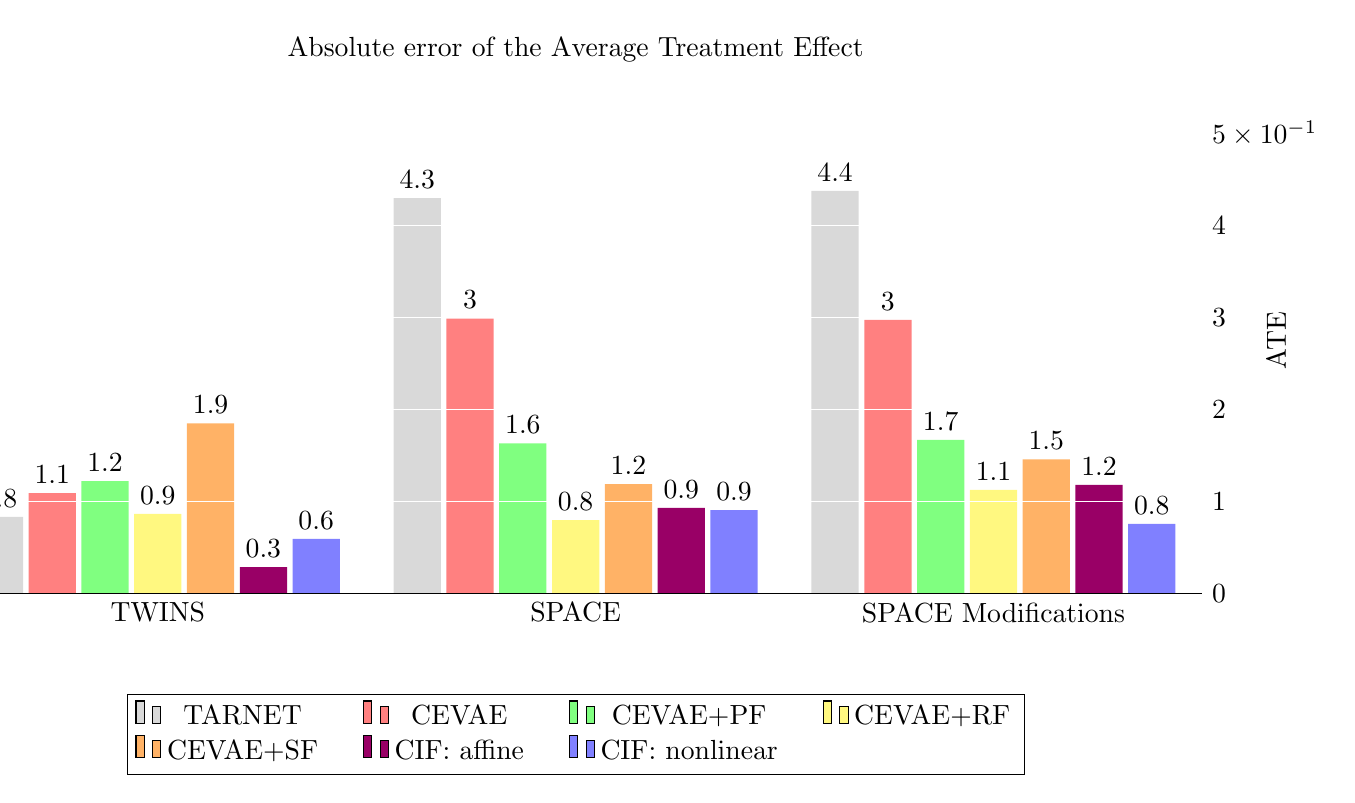
\begin{tikzpicture}[trim left=1cm]
    % \centering
    \begin{axis}[
        ybar, axis on top,
        title={Absolute error of the Average Treatment Effect},
        height=8cm, width=17.5cm,
        bar width=0.6cm,
        % bar shift=-0.3,
        xtick=data,
        ymajorgrids, tick align=inside,
        major grid style={draw=white},
        enlarge x limits=0.25,
        enlarge y limits={value=.1,upper},
        ymin=0, ymax=5,
        ytick={0, 1, 2, 3, 4, 5},
        yticklabels={0, 1, 2, 3, 4, $5\times10^{-1}$},
        axis x line*=bottom,
        axis y line*=right,
        y axis line style={opacity=0},
        tickwidth=0pt,
        % enlarge x limits=true,
        legend style={
            at={(0.5,-0.2)},
            anchor=north,
            legend columns=4,
            /tikz/every even column/.append style={column sep=0.5cm}
        },
        ylabel shift=-25pt,
        ylabel={ATE},
        symbolic x coords={
           TWINS, SPACE, SPACE Modifications},
        nodes near coords={
        \pgfmathprintnumber[precision=1, fixed]{\pgfplotspointmeta}
       }
    ]
    \addplot [draw=none, fill=gray!30] coordinates {
      (TWINS, 0.83) 
      (SPACE, 4.30)
      (SPACE Modifications, 4.38)};
    \addplot [draw=none,fill=red!50] coordinates {
      (TWINS, 1.09) 
      (SPACE, 2.99)
      (SPACE Modifications, 2.975)};
    \addplot [draw=none, fill=green!50] coordinates {
      (TWINS, 1.22) 
      (SPACE, 1.63)
      (SPACE Modifications, 1.67)};
    \addplot [draw=none, fill=yellow!50] coordinates {
      (TWINS, 0.864) 
      (SPACE, 0.796)
      (SPACE Modifications, 1.124)};
    \addplot [draw=none, fill=orange!60] coordinates {
      (TWINS, 1.85) 
      (SPACE, 1.189)
      (SPACE Modifications, 1.458)};
    \addplot [draw=none, fill=red!60!blue] coordinates {
      (TWINS, 0.285) 
      (SPACE, 0.930)
      (SPACE Modifications, 1.18)};
    \addplot [draw=none, fill=blue!50] coordinates {
      (TWINS, 0.591) 
      (SPACE, 0.904)
      (SPACE Modifications, 0.756)};
    \legend{TARNET, CEVAE, CEVAE+PF, CEVAE+RF, CEVAE+SF, CIF: affine, CIF: nonlinear}
    % \node[draw=black, fill=white] (a) at (13,730) {$6+$};
    \end{axis}
\end{tikzpicture}
\caption{Average Treatment effect scores for all models. Best viewed in colour. Lower score is better. Vertical axis is ranged from zero to $0.5$ for readability. The SPACE Modifications data is the average over all three distributional shifts of the Space Shapes dataset. The standard deviation for all models was approximately $10^{-2}$}
\label{fig:ATE}
\end{figure}


\section{Twins dataset}
For the Twins mortality prediction task, the CIF model makes a significant improvement over other models (see Figure \ref{fig:ATE}), especially so when using affine coupling layers. All CEVAE extensions perform worse, even worse than TARNet. However, on the Individual Treatment Effect, as seen in Figure \ref{fig:ITE}, both the original CEVAE and the extension with Planar Flow score significantly better than both TARNet and both the CIF versions. Again, the Radial Flow and Sylvester Flow extension perform poorly. This can be explained by the fact that both these models were able to achieve far better likelihood scores and were potentially overfitting, even in cases with a single flow. The Precision in Estimation of the Heterogeneous Effect does not show any significant difference between any of the models, as can be seen in Figure \ref{fig:PEHE}. The combined performance on all three metrics indicate that the CIF performs best at this task.

\setlength{\belowcaptionskip}{-5pt}

\begin{figure}
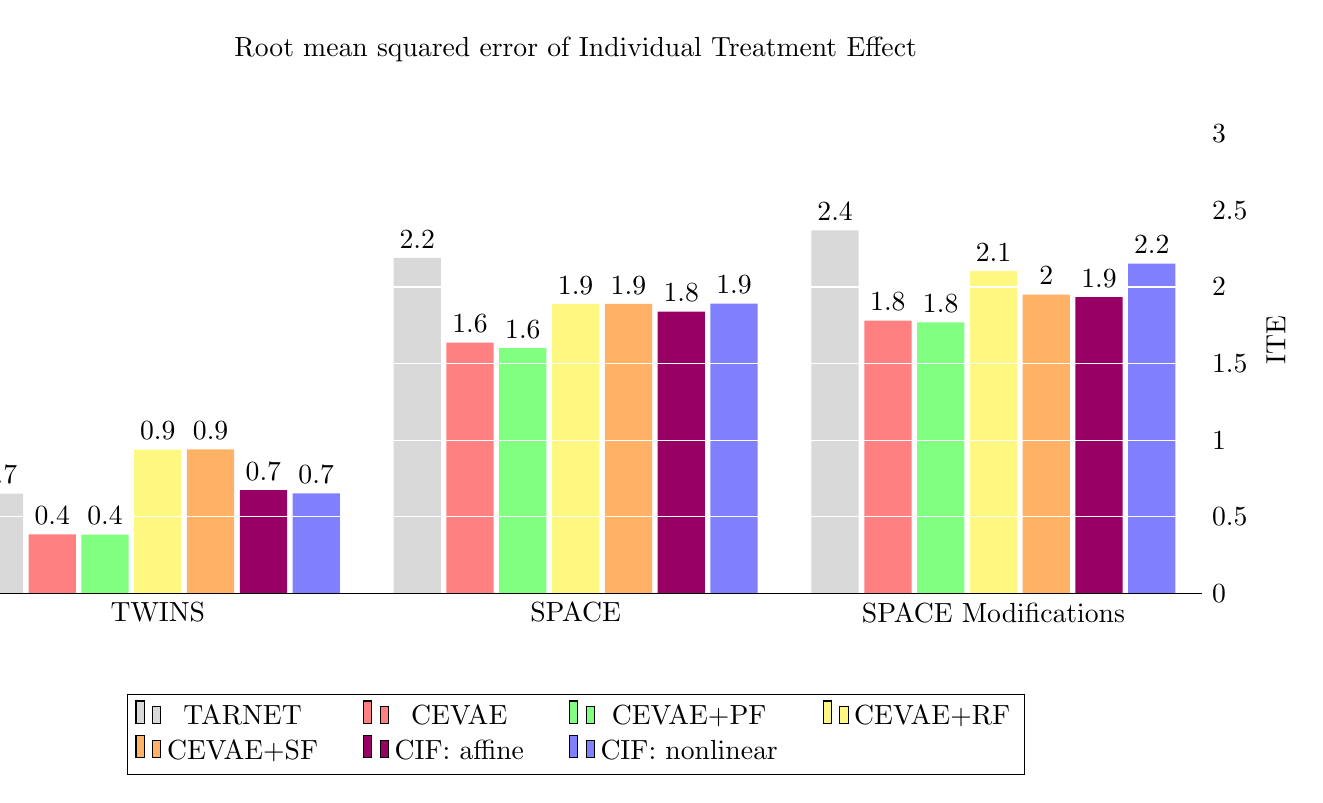
\begin{tikzpicture}[trim left=1cm]
    % \centering
    \begin{axis}[
        ybar, axis on top,
        title={Root mean squared error of Individual Treatment Effect},
        height=8cm, width=17.5cm,
        bar width=0.6cm,
        % bar shift=-0.3,
        xtick=data,
        ymajorgrids, tick align=inside,
        major grid style={draw=white},
        enlarge x limits=0.25,
        enlarge y limits={value=.1,upper},
        ymin=0, ymax=3,
        ytick={0, 0.5, 1, 1.5, 2, 2.5, 3},
        % yticklabels={0, 1, 2, 3, 4, 5, $6$},
        axis x line*=bottom,
        axis y line*=right,
        y axis line style={opacity=0},
        tickwidth=0pt,
        % enlarge x limits=true,
        legend style={
            at={(0.5,-0.2)},
            anchor=north,
            legend columns=4,
            /tikz/every even column/.append style={column sep=0.5cm}
        },
        ylabel={ITE},
        symbolic x coords={
           TWINS, SPACE, SPACE Modifications},
       nodes near coords={
        \pgfmathprintnumber[precision=1, fixed]{\pgfplotspointmeta}
       }
    ]
    \addplot [draw=none, fill=gray!30] coordinates {
      (TWINS, 0.65) 
      (SPACE, 2.19)
      (SPACE Modifications, 2.37)};
    \addplot [draw=none,fill=red!50] coordinates {
      (TWINS, 0.384) 
      (SPACE, 1.637)
      (SPACE Modifications, 1.78)};
    \addplot [draw=none, fill=green!50] coordinates {
      (TWINS, 0.383) 
      (SPACE, 1.601)
      (SPACE Modifications, 1.769)};
    \addplot [draw=none, fill=yellow!50] coordinates {
      (TWINS, 0.938) 
      (SPACE, 1.890)
      (SPACE Modifications, 2.104)};
    \addplot [draw=none, fill=orange!60] coordinates {
      (TWINS, 0.94) 
      (SPACE, 1.890)
      (SPACE Modifications, 1.95)};
    \addplot [draw=none, fill=red!60!blue] coordinates {
      (TWINS, 0.673) 
      (SPACE, 1.839)
      (SPACE Modifications, 1.934)};
    \addplot [draw=none, fill=blue!50] coordinates {
      (TWINS, 0.652) 
      (SPACE, 1.891)
      (SPACE Modifications, 2.152)};
    \legend{TARNET, CEVAE, CEVAE+PF, CEVAE+RF, CEVAE+SF, CIF: affine, CIF: nonlinear}
    \end{axis}
\end{tikzpicture}
\caption{Individual Treatment effect scores for all models. Best viewed in colour. Lower score is better. The SPACE Modifications data is the average over all three distributional shifts of the Space Shapes dataset. The standard deviation for all models was approximately $10^{-1}$}
\label{fig:ITE}
\end{figure}

\section{Space Shapes dataset}
The results on the Space Shapes dataset show a clear difference between the considered models. On the PEHE scores in Figure \ref{fig:PEHE}, there is almost an order of magnitude difference between TARNet and the CIF, and a difference of a factor four between the CEVAE and the CIF. The CEVAE does slightly better in terms of the ITE score, tied with the CEVAE with Planar Flow extension. The CEVAE with Radial Flow performs far better compared to the other two datasets, even achieving comparable scores to the CIF on all metrics. In contrast to the other datasets, the CEVAE with the Sylvester Flow extension shows an improvement over the CEVAE.

% The Sylvester Flow extension of the CEVAE does not as bad as on the other datasets, improving on the CEVAE.

\subsection{Performance decline due to distribution shift}\label{section:res_space_mod}
For the three post-training modifications we show the averaged scores of all three modifications, since there is very little variation in between then. Complete numbers are available in Appendix \ref{appendix:results}. The decrease in performance due to the modifications on the Space Shapes dataset is for the majority of the models no more than ten percent. On the Average Treatment Effect, we see that it is even less (see Figure \ref{fig:ATE}). The exception is the CEVAE with Radial Flow extension. The ATE score decreased with more than thirty percent, resulting in this model being surpassed in performance by the CIF with nonlinear couplings.

Surprisingly, the nonlinear CIF reaches a better ATE than on the original Space Shapes data of twenty percent, averaged over all three modifications. There doesn't seem to be an outlier in one of the modifications that was in some way easier than the original task. This effect is also seen in the PEHE scores; the increase in this score is ten percent. A hypothesis is that the modifications make the prediction task easier. However, none of the other tested models exhibit this performance increase, meaning it is not immediately likely that all three additional tasks are in general easier than the original prediction task.

For this experiment it is also the case that the CEVAE and CEVAE with Planar Flow achieved the best ITE, leading to the fact that these two models scored the best ITE in all experiments. But these two models did not reach comparable scores for the ATE and PEHE. The addition of the Planar Flow yielded better results on the Space Shapes data and its extensions.
%  - Most models don't deteriorate by a lot when looking at the SPACE Modifications data. Full results show that there is in general a slight improvement when having less objects in the scene. Fewer potential collisions and less gravity to consider.
%  - TARNet does obviously worse for space data, though it does okay for the TWINS data
%  - CEVAE and CEVAE + PF have the best ITE in all cases, also IHDP.
%  - Both CIF models are clearly best, though radial flow seems to do well on some metrics and not so well on others.
%  - Which models are overfitting? 

%ATE:: orig:1.82  avg diff comb: 1.88, avg diff num: 1.88, diff size: 2.04
\setlength{\belowcaptionskip}{0pt}


\begin{figure}
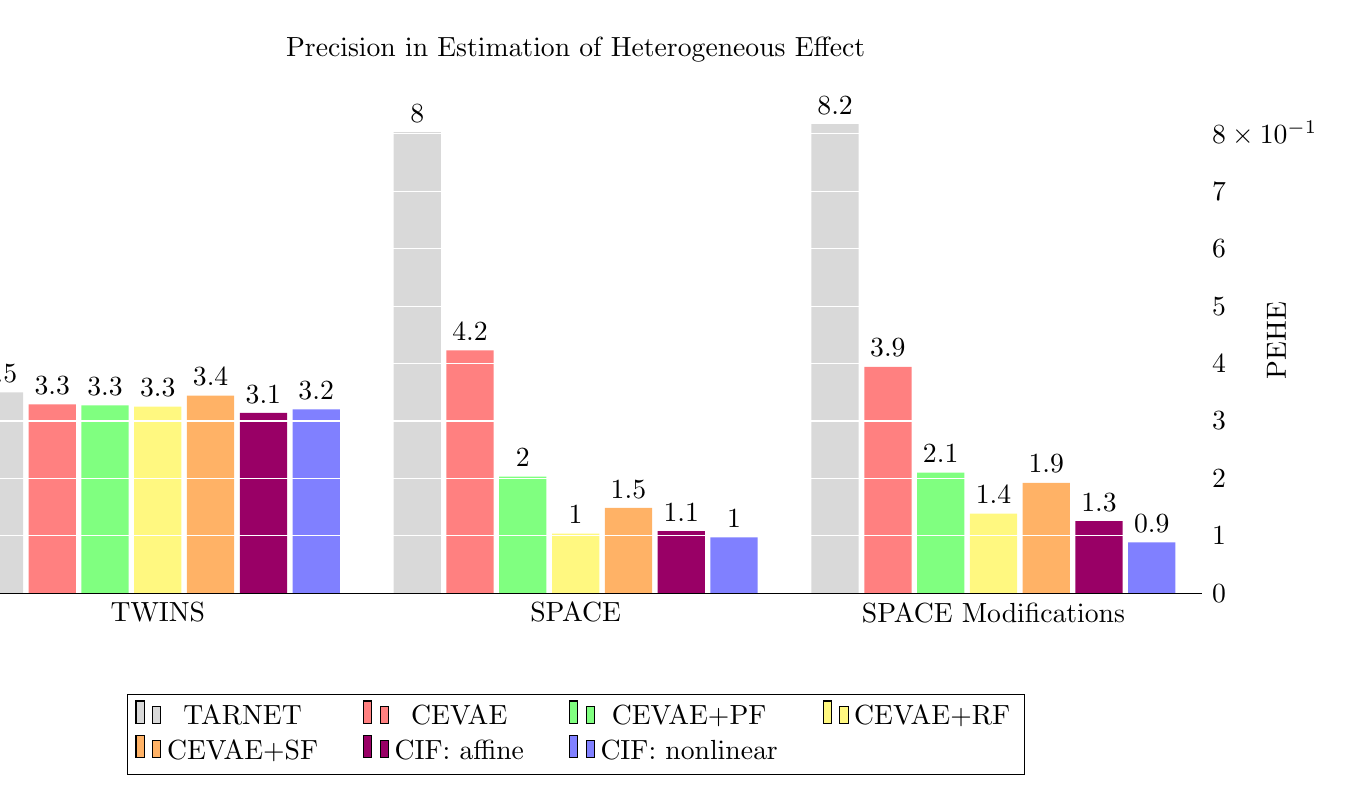
\begin{tikzpicture}[trim left=1cm]
    % \centering
    \begin{axis}[
        ybar, axis on top,
        title={Precision in Estimation of Heterogeneous Effect},
        height=8cm, width=17.5cm,
        bar width=0.6cm,
        % bar shift=-0.3,
        xtick=data,
        ymajorgrids, tick align=inside,
        major grid style={draw=white},
        enlarge x limits=0.25,
        enlarge y limits={value=.1,upper},
        ymin=0, ymax=8,
        ytick={0, 1, 2, 3, 4, 5, 6, 7, 8},
        yticklabels={0, 1, 2, 3, 4, 5, 6, 7, $8\times10^{-1}$},
        axis x line*=bottom,
        axis y line*=right,
        y axis line style={opacity=0},
        tickwidth=0pt,
        % enlarge x limits=true,
        legend style={
            at={(0.5,-0.2)},
            anchor=north,
            legend columns=4,
            /tikz/every even column/.append style={column sep=0.5cm}
        },
        ylabel shift=-25pt,
        ylabel={PEHE},
        symbolic x coords={
           TWINS, SPACE, SPACE Modifications},
       nodes near coords={
        \pgfmathprintnumber[precision=1, fixed]{\pgfplotspointmeta}
       }
    ]
    \addplot [draw=none, fill=gray!30] coordinates {
      (TWINS, 3.50) 
      (SPACE, 8.03)
      (SPACE Modifications, 8.17)};
    \addplot [draw=none,fill=red!50] coordinates {
      (TWINS, 3.29) 
      (SPACE, 4.23)
      (SPACE Modifications, 3.944)};
    \addplot [draw=none, fill=green!50] coordinates {
      (TWINS, 3.27) 
      (SPACE, 2.03)
      (SPACE Modifications, 2.099)};
    \addplot [draw=none, fill=yellow!50] coordinates {
      (TWINS, 3.25) 
      (SPACE, 1.04)
      (SPACE Modifications, 1.385)};
    \addplot [draw=none, fill=orange!60] coordinates {
      (TWINS, 3.44) 
      (SPACE, 1.486)
      (SPACE Modifications, 1.924)};
    \addplot [draw=none, fill=red!60!blue] coordinates {
      (TWINS, 3.14) 
      (SPACE, 1.08)
      (SPACE Modifications, 1.255)};
    \addplot [draw=none, fill=blue!50] coordinates {
      (TWINS, 3.20) 
      (SPACE, 0.971)
      (SPACE Modifications, 0.887)};
    \legend{TARNET, CEVAE, CEVAE+PF, CEVAE+RF, CEVAE+SF, CIF: affine, CIF: nonlinear}
    \end{axis}
\end{tikzpicture}
\caption{Precision in Estimation of Heterogeneous Effect for all models. Best viewed in colour. Lower score is better. The SPACE Modifications data is the average over all three distributional shifts of the Space Shapes dataset. The standard deviation for all models was approximately $10^{-2}$}
\label{fig:PEHE}
\end{figure}


%%%%%%%%%%%%%%%%%%%%%%%%%%%%%%%%%%%%%%%%%%%%%%%%%%%%%%%%%%%%%%%%%%%%%%%%%%%%%%%%
\chapter{Discussion and Conclusion}

\section{Conclusion}
Overall we can conclude that the Causal Inference Flow performed well on the tasks as they were defined. Although it did not reach the best scores on every metric on every dataset, it did so for the majority, and was worst in none of the tasks. Only on the low-dimensional IHDP dataset did other models show an advantage over the CIF models.

No clear conclusion can be draw if either the affine coupling or the nonlinear coupling works best in general. In all cases the scores of the two models were quite similar and the number of experiments in which one was significantly better than the other is roughly equal. There is also not a clear pattern in which model is better suited for which metric. 

The extensions of the CEVAE gave mixed results. What we can conclude is that the Sylvester Flow is not well suited for this type of predictions. What could be a possible explanation for that is the fact this the Sylvester Flow does not amortise its flow parameters but uses a hyper network to predict them for each sample separately. This has the potential to overfit when it extrapolates to new intervention-proxy combinations. Such overfitting effects due to more flexibility should reduce when the size of the dataset and dimensionality of the data increases, which is partially the case. The worst scores were reached on the smallest dataset (IHDP), so that would be a reasonable explanation. However, all models that were tested had more trainable parameters than the IHDP dataset, as mentioned in section \ref{section:data_space}, but not all of them suffered from such overfitting.

Nevertheless, the Planar Flow extension is a clear improvement on the CEVAE. It performed equal or better in all experiments, with the most significant improvement in the most complex dataset. From all this, we can conclude that a more flexible posterior does lead to better causal effect inference, with the caveat that not all normalising flow models are appropriate choices to do so.

The post-training modifications did not give as much insight in the performance of the models as expected. This is mostly due to the fact that all modifications resulted in roughly the same scores. Nevertheless, the results of the Space Shapes dataset showed the most explicit difference between the models. Therefore, we conclude that as a whole, the Space Shapes dataset did show which models were capable of handling more complex, high dimensional data.

\section{Discussion}
Although we were able to give a positive answer to both of the research questions, they are not without caveats. Firstly we have the fact that it is not entirely clear why some models do well on one metric and not so well on others. Moreover, there does not seem to be a clear pattern which model does better on which metric.


The Space Shapes dataset and the experiments performed on it have some uncertain components to them. The generalisation that was chosen for the metrics has some arbitrariness to it. We chose two values for the intervention distribution to get a binary difference, but there was no mathematical foundation for the choice of these two values. Additionally, there is the issue of applying this principle to other datasets with no clear binary intervention. It poses problems if we would want to use it in an empirical study due to ethical concerns. Administering a random dose of a drug to a patient would not go down well with the ethics committee, regardless of the potential profit of such an experiment.

Another point that calls for consideration is the implicit assumption that was made that the increased complexity of the Space Shapes dataset originated in some real-world problem with comparable complexity, but this has not yet been shown.

% Does making the proxy more complex say something interesting?


% Not obvious why in some metrics one model is better and on another metric another metric is better.

% Have some models just ignored the other shapes and learned the distance from the Space Ship to the right of the image?

Looking at the broader picture leads us to a general concern in the way this causal inference approach could be used in practice. As we have discussed, validation of a model always requires counterfactual information, which can only be available in simulated data. This means that any prediction based on real data can not be verified. Therefore, an empirical experiment would always be needed to verify prediction results.



\subsection{Future work}
In the results in section \ref{section:res_space_mod}, we saw that the modifications on the Space Shapes dataset led in a few cases to improvement of the score. This is quite counter-intuitive when we change the test data compared to the training data. What might be an explanation, is that the 'unmodified' data contained the hardest problem of the four. If we were to train and test each model on these four datasets separately this hypothesis could be tested.

The Space Shapes dataset purposefully contains more hyperparameters to vary than were adapted in this thesis, such as image resolution and image size. Changing these two hyperparameters also allows more potential values for the other hyperparameters (a larger image has a higher potential number of objects). A more extensive pass over these hyperparameters could lead to more insights on causal effect inference models.

Lastly, we chose to keep the core architecture of all models from earlier work the same, but these could potentially be optimised for better performance.

% Do a more extensive sweep over the hyperparameters/network architecture. 
% The different types of flow models showed a great variety in experimental results.
% Inverse Autoregressive Flow?
% Change size of image in Space dataset to give more options with number of objects
% Increase resolution of image.
% The two intervention distributions we compare are chosen somewhat arbitrary. To get more conclusive results, more distributions have to be compared.





%%%%%%%%%%%%%%%%%%%%%%%%%%%%%%%%%%%%%%%%%%%%%%%%%%%%%%%%%%%%%%%%%%%%%%%%%%%%%%%%
% \bibliography{references.bib}
% \bibliographystyle{apalike}
\printbibliography[]

\begin{appendices}
\renewcommand{\arraystretch}{1.3}
\chapter{Generation process of the Space Shapes dataset}
\label{appendix:space_shapes}
The SPACE dataset is generated in several steps. Setting up all prior information, generating initial states, interventions and outcome states, and converting the used representation to images. For the first step the following hyperparameters are needed. All of these can be changed manually to create a slightly different dataset:
\begin{enumerate}
    \item Height and width of the scene as whole number. These two numbers determine the size of the grind in which the objects are placed. Their product cannot be lower than the total number of objects.
    \item Number of different colours and number of different shapes the objects can take. It is recommended that these two numbers are coprime as to allow the most actually different looking objects.
    \item Total number of different objects that can exist. This can at most be the number of colours times the number of shapes, if those two numbers are coprime. Otherwise the maximum has to be divided by their common divisors.
    \item Colour scale factor and shape scale factor. These two factors determine the difference in scaling the prior of the gravity differs between object of a different colour and objects of a different shapes respectively.
    \item The 'prior' dimensions, used for sampling the prior of all values
    \item Scoring scale. Linearly scales to final Score determines its upper limit
\end{enumerate}
The generation process works as follows. First the gravity per object is generated:

\begin{align}
    colour factor_c &= \left(1 + \frac{c \times colour scale factor}{\# colours} \right)\\
    shape factor_s &= \left(1 + \frac{s \times shape scale factor}{\#shapes}\right) \\
    gravity factor_n &= colour factor_n * shape factor_n \\
    gravity_n &\sim \Norm(gravity factor_n, 1)
\end{align}
Then we sample from the intervention prior and the positions prior:
\begin{align}
    I_M &\sim \Norm(0, I)\\
    P_M &\sim \Norm(0, I)\\
    prior &\sim \Norm(0, I)\\
    Prior &= \begin{pmatrix}gravity_1 \\ \vdots\\gravity_N \\ prior\end{pmatrix}\\
\end{align}
Next we use these priors to compute the weights of the distribution that governs the positions of the objects in the initial states and sample these positions:
\begin{align}
position_n \sim Mult(\sigma(Prior \cdot P_M)_n, 1)    
\end{align}
Then we calculate the Steering of the Space Ship:
\begin{equation}
    Steering = Prior \cdot I_m
\end{equation}
Ans use that to get the Movement of the Space Ship
\begin{align}
    distance_n &= position_n - position_0\\
    direction &= Steering +\sum\limits^N_{n=1} distance_n * gravity_n\\
    new\_position &= position_0 + direction
\end{align}
Lastly we calculate the score as follows:
\begin{equation}
    score = score\_scale \times \frac{1 - ||new\_position - goal ||_2}{\sqrt{(width - 1)^2 + (height-1)^2}}
\end{equation}


\chapter{Architecture of networks used}\label{appendix:architecture}
Most models described in this paper use several neural networks as components of the larger model. Their exact architectures are described here.

\section*{Convolutional networks}
Each network that has images as input uses the same convolutional network architecture, as can be seen in Figure \ref{fig:conv_net}. This consists of blocks with a batch normalisation, exponential linear unit and convolutional layer. Furthermore, the model has several skip connections between each set of three blocks.

\section*{Fully connected networks}
All other neural networks take (abstract) feature vectors as input. These networks are set up as fully connected networks with exponential linear units as nonlinearities.

\begin{figure}
    \centering
    \includestandalone[]{Figures/conv_res_net}
    \hspace{1cm}
    \includestandalone[]{Figures/conv_block}
    \caption{Convolutional residual network that is used on the left. The Block components are shown in full on the right.}
    \label{fig:conv_net}
\end{figure}

\chapter{Raw data of experiments}
\label{appendix:results}
\begin{figure}
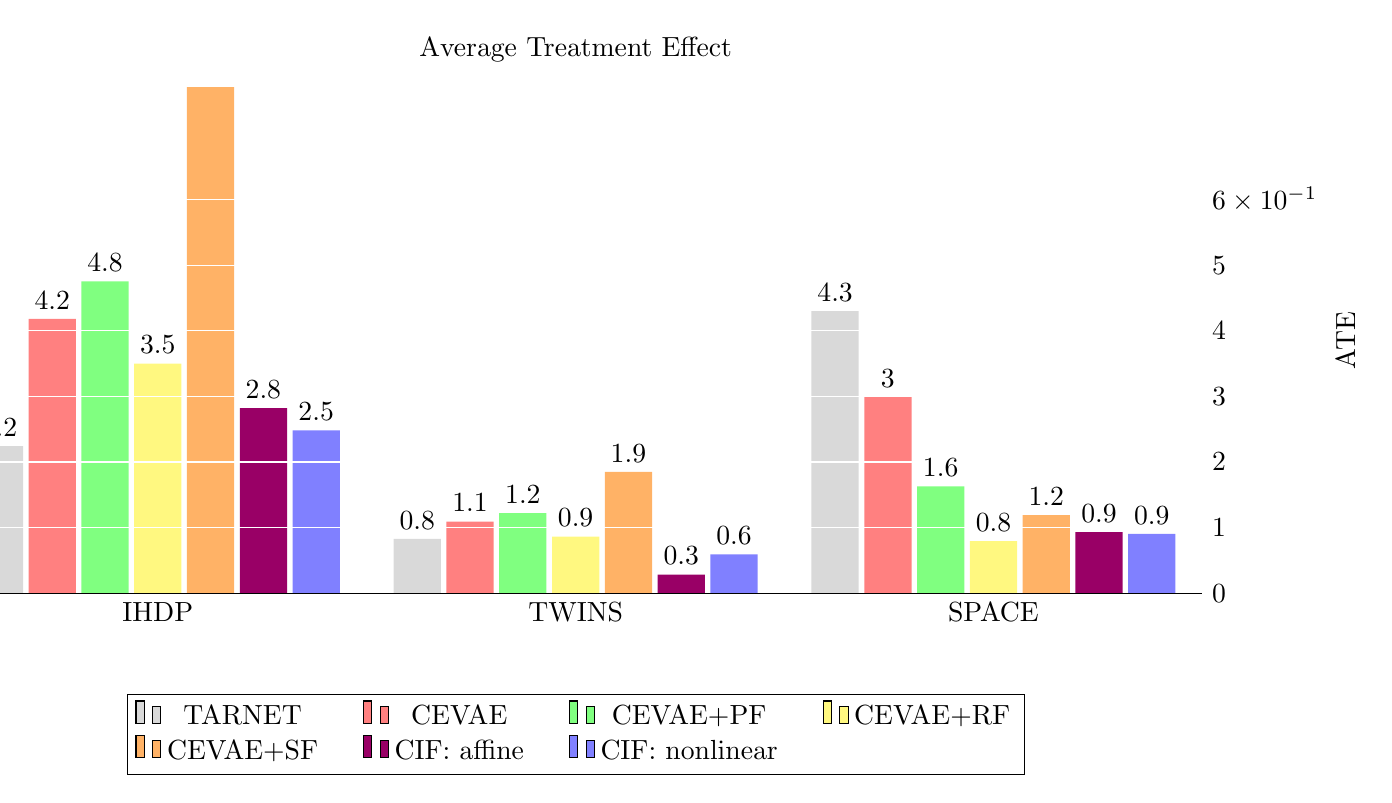
\begin{tikzpicture}[trim left=1cm]
    % \centering
    \begin{axis}[
        ybar, axis on top,
        title={Average Treatment Effect},
        height=8cm, width=17.5cm,
        bar width=0.6cm,
        % bar shift=-0.3,
        xtick=data,
        ymajorgrids, tick align=inside,
        major grid style={draw=white},
        enlarge x limits=0.25,
        enlarge y limits={value=.1,upper},
        ymin=0, ymax=7,
        ytick={0, 1, 2, 3, 4, 5, 6},
        yticklabels={0, 1, 2, 3, 4, 5, $6\times10^{-1}$},
        axis x line*=bottom,
        axis y line*=right,
        y axis line style={opacity=0},
        tickwidth=0pt,
        % enlarge x limits=true,
        legend style={
            at={(0.5,-0.2)},
            anchor=north,
            legend columns=4,
            /tikz/every even column/.append style={column sep=0.5cm}
        },
        ylabel={ATE},
        symbolic x coords={
           IHDP, TWINS, SPACE},
        nodes near coords={
        \pgfmathprintnumber[precision=1, fixed]{\pgfplotspointmeta}
       }
    ]
    \addplot [draw=none, fill=gray!30] coordinates {
      (IHDP, 2.24)
      (TWINS, 0.83) 
      (SPACE, 4.3)};
    \addplot [draw=none,fill=red!50] coordinates {
      (IHDP, 4.18)
      (TWINS, 1.09) 
      (SPACE, 2.99)};
    \addplot [draw=none, fill=green!50] coordinates {
      (IHDP, 4.75)
      (TWINS, 1.22) 
      (SPACE, 1.63)};
    \addplot [draw=none, fill=yellow!50] coordinates {
      (IHDP, 3.50)
      (TWINS, 0.864) 
      (SPACE, 0.796)};
    \addplot [draw=none, fill=orange!60] coordinates {
      (IHDP, 11.9)
      (TWINS, 1.85) 
      (SPACE, 1.189)};
    \addplot [draw=none, fill=red!60!blue] coordinates {
      (IHDP, 2.82)
      (TWINS, 0.285) 
      (SPACE, 0.930)};
    \addplot [draw=none, fill=blue!50] coordinates {
      (IHDP, 2.48)
      (TWINS, 0.591) 
      (SPACE, 0.904)};
    \legend{TARNET, CEVAE, CEVAE+PF, CEVAE+RF, CEVAE+SF, CIF: affine, CIF: nonlinear}
    % \node[draw=black, fill=white] (a) at (13,730) {$6+$};
    \end{axis}
\end{tikzpicture}
\caption{Average Treatment effect scores for all models. Vertical axis is ranged from zero to $0.6$  for readability. Lower score is better.}
\end{figure}


\begin{figure}
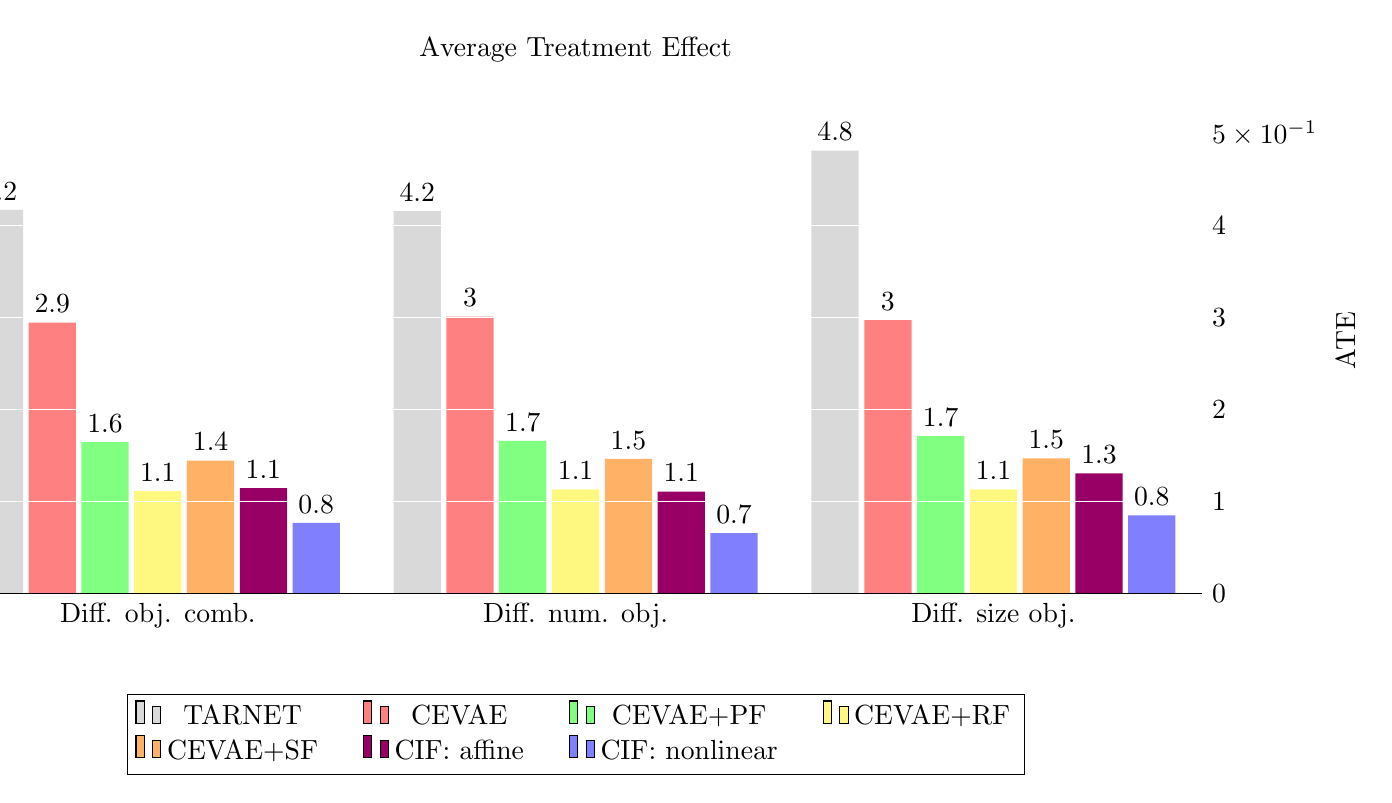
\begin{tikzpicture}[trim left=1cm]
    % \centering
    \begin{axis}[
        ybar, axis on top,
        title={Average Treatment Effect},
        height=8cm, width=17.5cm,
        bar width=0.6cm,
        % bar shift=-0.3,
        xtick=data,
        ymajorgrids, tick align=inside,
        major grid style={draw=white},
        enlarge x limits=0.25,
        enlarge y limits={value=.1,upper},
        ymin=0, ymax=5,
        ytick={0, 1, 2, 3, 4, 5},
        yticklabels={0, 1, 2, 3, 4, $5\times10^{-1}$},
        axis x line*=bottom,
        axis y line*=right,
        y axis line style={opacity=0},
        tickwidth=0pt,
        % enlarge x limits=true,
        legend style={
            at={(0.5,-0.2)},
            anchor=north,
            legend columns=4,
            /tikz/every even column/.append style={column sep=0.5cm}
        },
        ylabel={ATE},
        symbolic x coords={
           Diff. obj. comb., Diff. num. obj., Diff. size obj.},
       nodes near coords={
        \pgfmathprintnumber[precision=1, fixed]{\pgfplotspointmeta}
       }
    ]
    \addplot [draw=none, fill=gray!30] coordinates {
      (Diff. obj. comb., 4.171)
      (Diff. num. obj., 4.158) 
      (Diff. size obj., 4.816)};
    \addplot [draw=none,fill=red!50] coordinates {
      (Diff. obj. comb., 2.945)
      (Diff. num. obj., 3.011) 
      (Diff. size obj., 2.972)};
    \addplot [draw=none, fill=green!50] coordinates {
      (Diff. obj. comb., 1.645)
      (Diff. num. obj., 1.657) 
      (Diff. size obj., 1.710)};
    \addplot [draw=none, fill=yellow!50] coordinates {
      (Diff. obj. comb., 1.111)
      (Diff. num. obj., 1.130) 
      (Diff. size obj., 1.131)};
    \addplot [draw=none, fill=orange!60] coordinates {
      (Diff. obj. comb., 1.444)
      (Diff. num. obj., 1.462) 
      (Diff. size obj., 1.469)};
    \addplot [draw=none, fill=red!60!blue] coordinates {
      (Diff. obj. comb., 1.143)
      (Diff. num. obj., 1.106) 
      (Diff. size obj., 1.305)};
    \addplot [draw=none, fill=blue!50] coordinates {
      (Diff. obj. comb., 0.767)
      (Diff. num. obj., 0.655) 
      (Diff. size obj., 0.847)};
    \legend{TARNET, CEVAE, CEVAE+PF, CEVAE+RF, CEVAE+SF, CIF: affine, CIF: nonlinear}
    \end{axis}
\end{tikzpicture}
\caption{Average Treatment Effect for all models. Deviations of the SPACE dataset. Lower score is better.}
\end{figure}


\begin{figure}
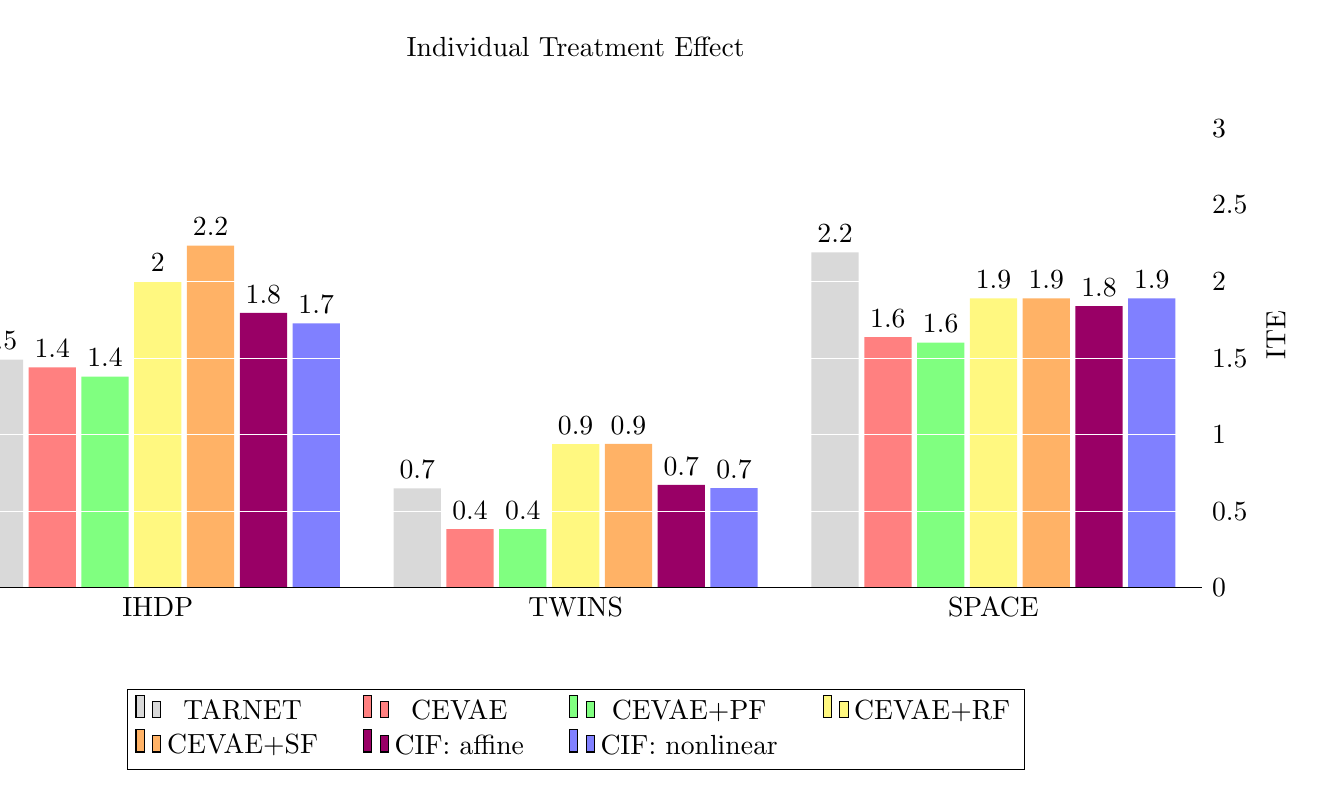
\begin{tikzpicture}[trim left=1cm]
    % \centering
    \begin{axis}[
        ybar, axis on top,
        title={Individual Treatment Effect},
        height=8cm, width=17.5cm,
        bar width=0.6cm,
        % bar shift=-0.3,
        xtick=data,
        ymajorgrids, tick align=inside,
        major grid style={draw=white},
        enlarge x limits=0.25,
        enlarge y limits={value=.1,upper},
        ymin=0, ymax=3,
        ytick={0, 0.5, 1, 1.5, 2, 2.5, 3},
        % yticklabels={0, 1, 2, 3, 4, 5, $6$},
        axis x line*=bottom,
        axis y line*=right,
        y axis line style={opacity=0},
        tickwidth=0pt,
        % enlarge x limits=true,
        legend style={
            at={(0.5,-0.2)},
            anchor=north,
            legend columns=4,
            /tikz/every even column/.append style={column sep=0.5cm}
        },
        ylabel={ITE},
        symbolic x coords={
           IHDP, TWINS, SPACE},
       nodes near coords={
        \pgfmathprintnumber[precision=1, fixed]{\pgfplotspointmeta}
       }
    ]
    \addplot [draw=none, fill=gray!30] coordinates {
      (IHDP, 1.49)
      (TWINS, 0.65) 
      (SPACE, 2.19)};
    \addplot [draw=none,fill=red!50] coordinates {
      (IHDP, 1.44)
      (TWINS, 0.384) 
      (SPACE, 1.637)};
    \addplot [draw=none, fill=green!50] coordinates {
      (IHDP, 1.379)
      (TWINS, 0.383) 
      (SPACE, 1.601)};
    \addplot [draw=none, fill=yellow!50] coordinates {
      (IHDP, 2.00)
      (TWINS, 0.938) 
      (SPACE, 1.890)};
    \addplot [draw=none, fill=orange!60] coordinates {
      (IHDP, 2.235)
      (TWINS, 0.94) 
      (SPACE, 1.890)};
    \addplot [draw=none, fill=red!60!blue] coordinates {
      (IHDP, 1.796)
      (TWINS, 0.673) 
      (SPACE, 1.839)};
    \addplot [draw=none, fill=blue!50] coordinates {
      (IHDP, 1.727)
      (TWINS, 0.652) 
      (SPACE, 1.891)};
    \legend{TARNET, CEVAE, CEVAE+PF, CEVAE+RF, CEVAE+SF, CIF: affine, CIF: nonlinear}
    \end{axis}
\end{tikzpicture}
\caption{Individual Treatment effect scores for all models. Lower score is better.}
\end{figure}

\begin{figure}
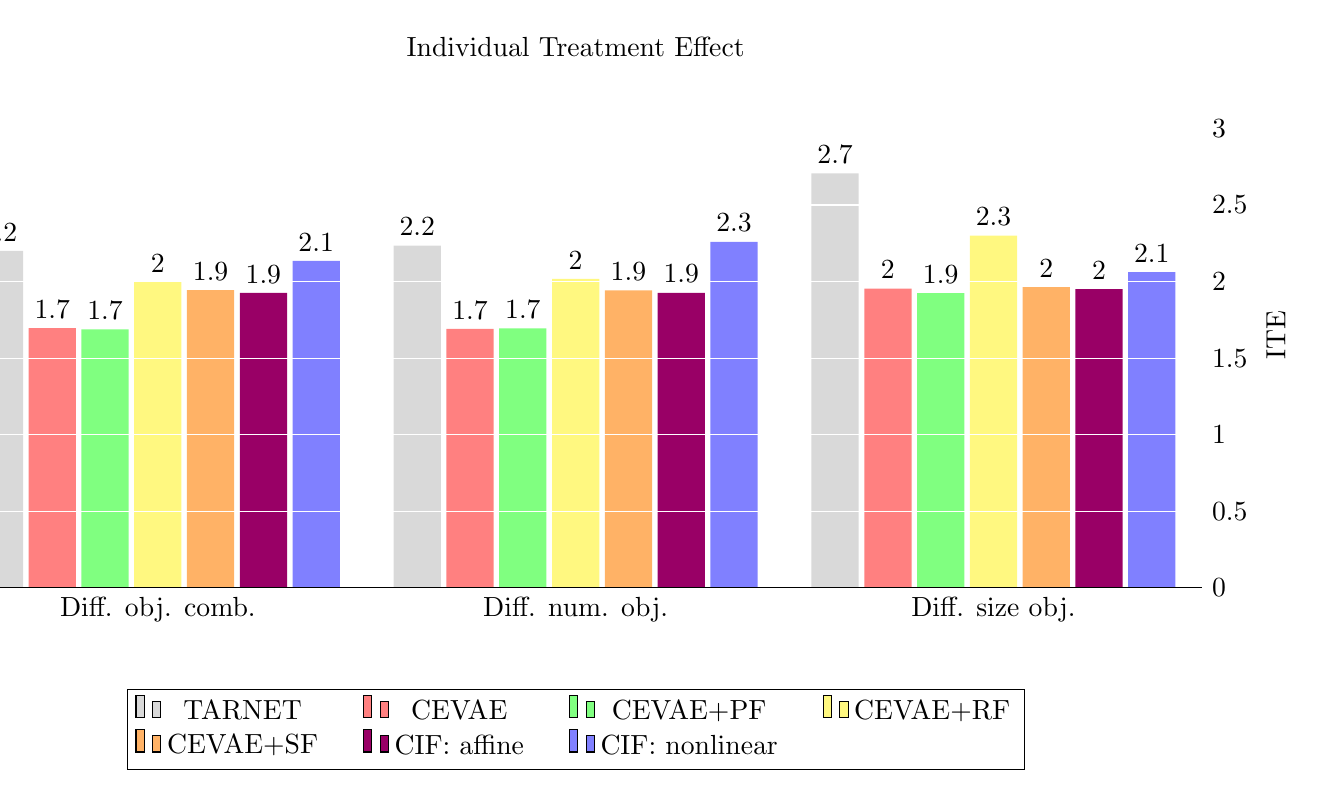
\begin{tikzpicture}[trim left=1cm]
    % \centering
    \begin{axis}[
        ybar, axis on top,
        title={Individual Treatment Effect},
        height=8cm, width=17.5cm,
        bar width=0.6cm,
        % bar shift=-0.3,
        xtick=data,
        ymajorgrids, tick align=inside,
        major grid style={draw=white},
        enlarge x limits=0.25,
        enlarge y limits={value=.1,upper},
        ymin=0, ymax=3,
        ytick={0, 0.5, 1, 1.5, 2, 2.5, 3},
        % yticklabels={0, 1, 2, 3, 4, $5\times10^{-1}$},
        axis x line*=bottom,
        axis y line*=right,
        y axis line style={opacity=0},
        tickwidth=0pt,
        % enlarge x limits=true,
        legend style={
            at={(0.5,-0.2)},
            anchor=north,
            legend columns=4,
            /tikz/every even column/.append style={column sep=0.5cm}
        },
        ylabel={ITE},
        symbolic x coords={
           Diff. obj. comb., Diff. num. obj., Diff. size obj.},
       nodes near coords={
        \pgfmathprintnumber[precision=1, fixed]{\pgfplotspointmeta}
       }
    ]
    \addplot [draw=none, fill=gray!30] coordinates {
      (Diff. obj. comb., 2.20)
      (Diff. num. obj., 2.235) 
      (Diff. size obj., 2.706)};
    \addplot [draw=none,fill=red!50] coordinates {
      (Diff. obj. comb., 1.696)
      (Diff. num. obj., 1.691) 
      (Diff. size obj., 1.954)};
    \addplot [draw=none, fill=green!50] coordinates {
      (Diff. obj. comb., 1.688)
      (Diff. num. obj., 1.695) 
      (Diff. size obj., 1.924)};
    \addplot [draw=none, fill=yellow!50] coordinates {
      (Diff. obj. comb., 1.996)
      (Diff. num. obj., 2.017) 
      (Diff. size obj., 2.300)};
    \addplot [draw=none, fill=orange!60] coordinates {
      (Diff. obj. comb., 1.945)
      (Diff. num. obj., 1.942) 
      (Diff. size obj., 1.963)};
    \addplot [draw=none, fill=red!60!blue] coordinates {
      (Diff. obj. comb., 1.926)
      (Diff. num. obj., 1.927) 
      (Diff. size obj., 1.951)};
    \addplot [draw=none, fill=blue!50] coordinates {
      (Diff. obj. comb., 2.135)
      (Diff. num. obj., 2.260) 
      (Diff. size obj., 2.062)};
    \legend{TARNET, CEVAE, CEVAE+PF, CEVAE+RF, CEVAE+SF, CIF: affine, CIF: nonlinear}
    \end{axis}
\end{tikzpicture}
\caption{Individual Treatment Effect for all models. Deviations of the SPACE dataset. Lower score is better.}
\end{figure}


\begin{figure}
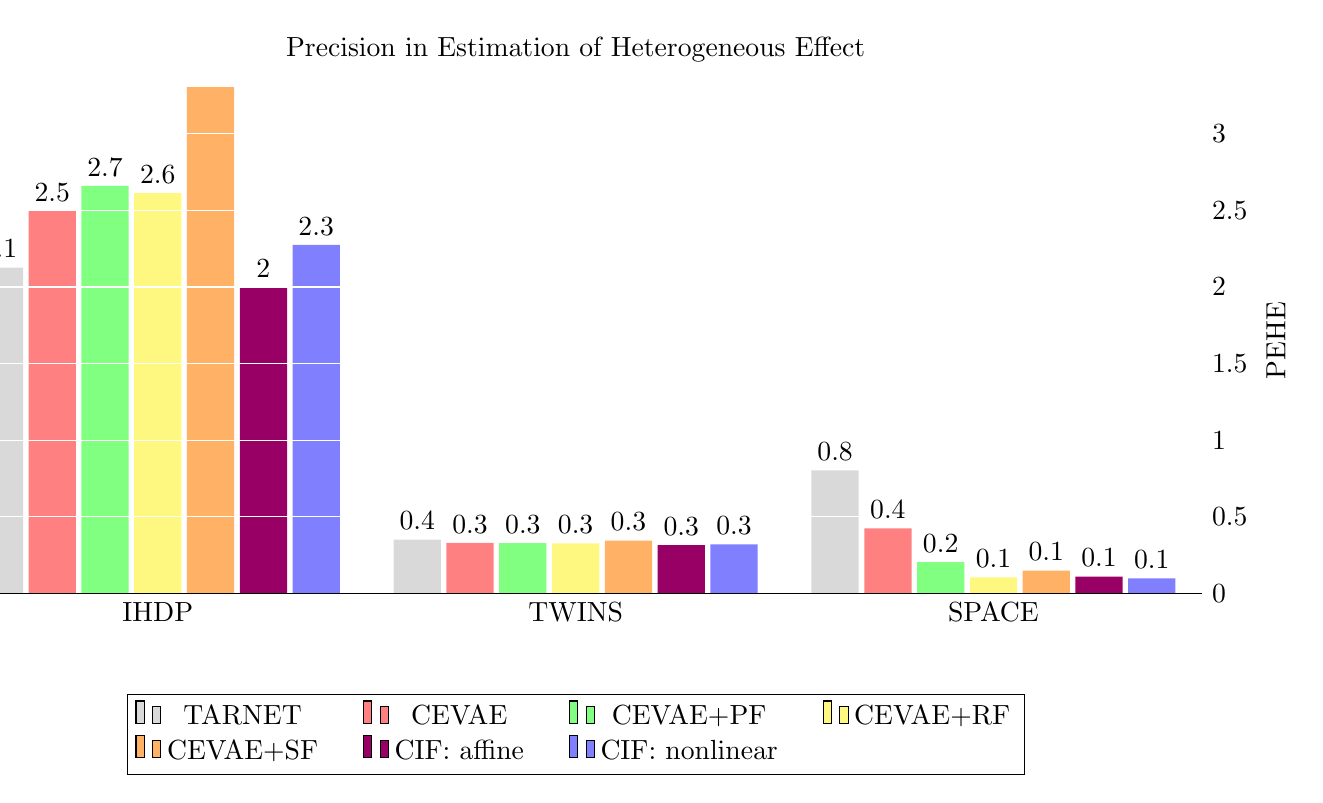
\begin{tikzpicture}[trim left=1cm]
    % \centering
    \begin{axis}[
        ybar, axis on top,
        title={Precision in Estimation of Heterogeneous Effect},
        height=8cm, width=17.5cm,
        bar width=0.6cm,
        % bar shift=-0.3,
        xtick=data,
        ymajorgrids, tick align=inside,
        major grid style={draw=white},
        enlarge x limits=0.25,
        enlarge y limits={value=.1,upper},
        ymin=0, ymax=3,
        ytick={0, 0.5, 1, 1.5, 2, 2.5, 3},
        % yticklabels={0, 1, 2, 3, 4, 5, $6$},
        axis x line*=bottom,
        axis y line*=right,
        y axis line style={opacity=0},
        tickwidth=0pt,
        % enlarge x limits=true,
        legend style={
            at={(0.5,-0.2)},
            anchor=north,
            legend columns=4,
            /tikz/every even column/.append style={column sep=0.5cm}
        },
        ylabel={PEHE},
        symbolic x coords={
           IHDP, TWINS, SPACE},
       nodes near coords={
        \pgfmathprintnumber[precision=1, fixed]{\pgfplotspointmeta}
       }
    ]
    \addplot [draw=none, fill=gray!30] coordinates {
      (IHDP, 2.126)
      (TWINS, 0.35) 
      (SPACE, 0.803)};
    \addplot [draw=none,fill=red!50] coordinates {
      (IHDP, 2.497)
      (TWINS, 0.329) 
      (SPACE, 0.423)};
    \addplot [draw=none, fill=green!50] coordinates {
      (IHDP, 2.66)
      (TWINS, 0.327) 
      (SPACE, 0.203)};
    \addplot [draw=none, fill=yellow!50] coordinates {
      (IHDP, 2.613)
      (TWINS, 0.325) 
      (SPACE, 0.104)};
    \addplot [draw=none, fill=orange!60] coordinates {
      (IHDP, 3.859)
      (TWINS, 0.344) 
      (SPACE, 0.1486)};
    \addplot [draw=none, fill=red!60!blue] coordinates {
      (IHDP, 1.995)
      (TWINS, 0.314) 
      (SPACE, 0.108)};
    \addplot [draw=none, fill=blue!50] coordinates {
      (IHDP, 2.275)
      (TWINS, 0.320) 
      (SPACE, 0.0971)};
    \legend{TARNET, CEVAE, CEVAE+PF, CEVAE+RF, CEVAE+SF, CIF: affine, CIF: nonlinear}
    \end{axis}
\end{tikzpicture}
\caption{Precision in Estimation of Heterogeneous Effect for all models. Lower score is better.}
\end{figure}


\begin{figure}
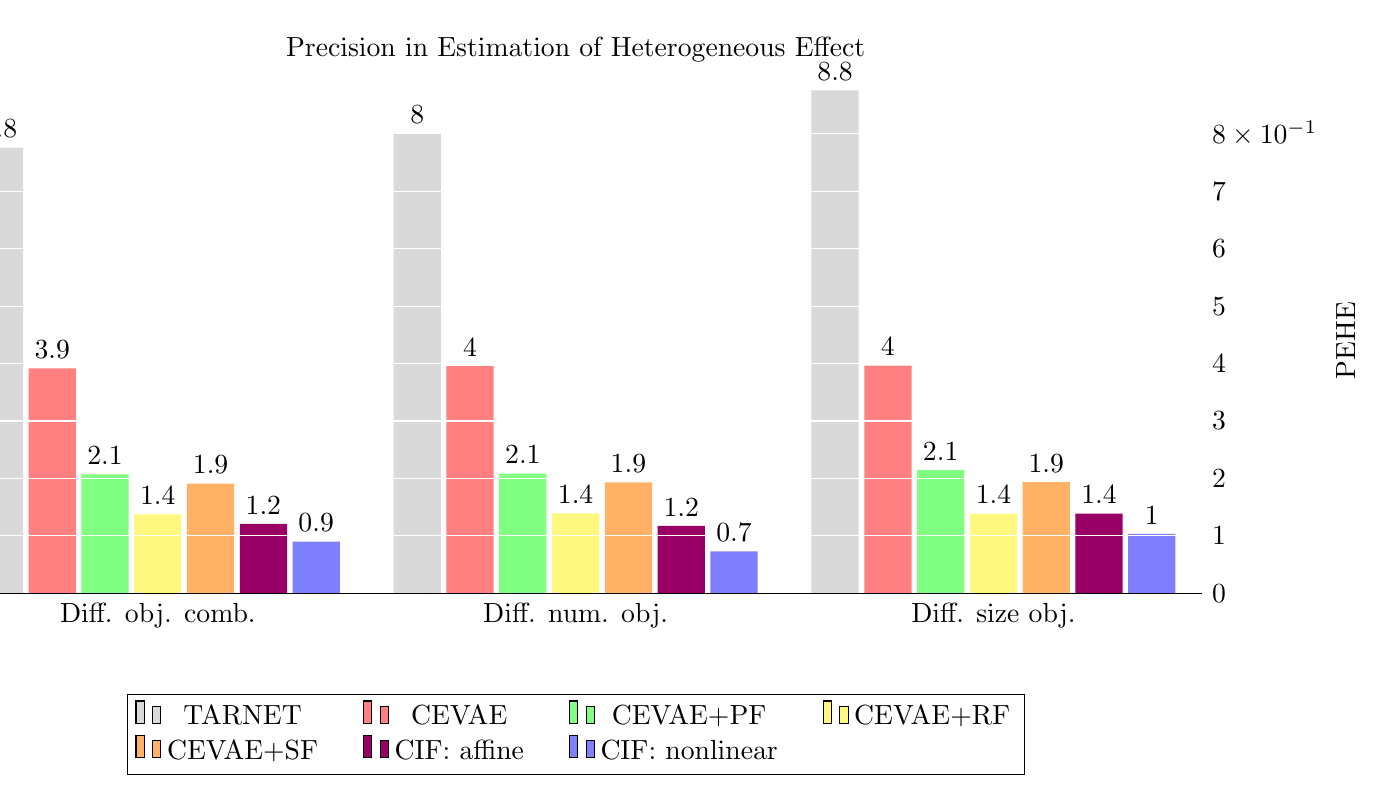
\begin{tikzpicture}[trim left=1cm]
    % \centering
    \begin{axis}[
        ybar, axis on top,
        title={Precision in Estimation of Heterogeneous Effect},
        height=8cm, width=17.5cm,
        bar width=0.6cm,
        % bar shift=-0.3,
        xtick=data,
        ymajorgrids, tick align=inside,
        major grid style={draw=white},
        enlarge x limits=0.25,
        enlarge y limits={value=.1,upper},
        ymin=0, ymax=8,
        ytick={0, 1, 2, 3, 4, 5, 6, 7, 8},
        yticklabels={0, 1, 2, 3, 4, 5, 6, 7, $8\times10^{-1}$},
        axis x line*=bottom,
        axis y line*=right,
        y axis line style={opacity=0},
        tickwidth=0pt,
        % enlarge x limits=true,
        legend style={
            at={(0.5,-0.2)},
            anchor=north,
            legend columns=4,
            /tikz/every even column/.append style={column sep=0.5cm}
        },
        ylabel={PEHE},
        symbolic x coords={
           Diff. obj. comb., Diff. num. obj., Diff. size obj.},
       nodes near coords={
        \pgfmathprintnumber[precision=1, fixed]{\pgfplotspointmeta}
       }
    ]
    \addplot [draw=none, fill=gray!30] coordinates {
      (Diff. obj. comb., 7.759)
      (Diff. num. obj., 8.006) 
      (Diff. size obj., 8.755)};
    \addplot [draw=none,fill=red!50] coordinates {
      (Diff. obj. comb., 3.914)
      (Diff. num. obj., 3.955) 
      (Diff. size obj., 3.963)};
    \addplot [draw=none, fill=green!50] coordinates {
      (Diff. obj. comb., 2.068)
      (Diff. num. obj., 2.085) 
      (Diff. size obj., 2.146)};
    \addplot [draw=none, fill=yellow!50] coordinates {
      (Diff. obj. comb., 1.372)
      (Diff. num. obj., 1.392) 
      (Diff. size obj., 1.388)};
    \addplot [draw=none, fill=orange!60] coordinates {
      (Diff. obj. comb., 1.908)
      (Diff. num. obj., 1.929) 
      (Diff. size obj., 1.936)};
    \addplot [draw=none, fill=red!60!blue] coordinates {
      (Diff. obj. comb., 1.208)
      (Diff. num. obj., 1.172) 
      (Diff. size obj., 1.385)};
    \addplot [draw=none, fill=blue!50] coordinates {
      (Diff. obj. comb., 0.898)
      (Diff. num. obj., 0.729) 
      (Diff. size obj., 1.035)};
    \legend{TARNET, CEVAE, CEVAE+PF, CEVAE+RF, CEVAE+SF, CIF: affine, CIF: nonlinear}
    \end{axis}
\end{tikzpicture}
\caption{Precision in Estimation of Heterogeneous Effect for all models. Deviations of the SPACE dataset. Lower score is better.}
\end{figure}


\begin{table}[h]
    \centering
    \begin{adjustbox}{center}
    \begin{tabular}{l||c|c|c||c|c|c||c|c|c|}
        %  & & IHDP & & & TWINS & & & SPACE &\\
        & \multicolumn{3}{|c||}{IHDP} & \multicolumn{3}{|c||}{TWINS} & \multicolumn{3}{|c|}{SPACE} \\ 
         Model & ATE & ITE & PEHE & ATE & ITE & PEHE & ATE & ITE & PEHE \\
         \hline \hline
         TARNET & $\mathbf{2.24\text{e-}}1$ & $1.490$ & 2.126 &   $8.3\text{e-}2$ & $6.51\text{e-}1$ & $3.50\text{e-}1$ &     $4.30\text{e-}1$ & 2.191 & $8.032\text{e-}1$\\
         \hline
         CEVAE & $4.18\text{e-}1$ & 1.443 & 2.497 &    $1.09\text{e-}1$ & $\mathbf{3.84\textbf{e-}1}$ & $3.29\text{e-}1$ & $2.99\text{e-}1$ & 1.637 & $4.23\text{e-}1$\\
         \hline
         CEVAE + PF & $4.75\text{e-}1$ & $\mathbf{1.379}$ &  2.662 & $1.22\text{e-}1$ & $\mathbf{3.83\text{\text{e-}}1}$ & $3.27\text{e-}1$ & $1.63\text{e-}1$ & $\mathbf{1.601}$ & $2.03\text{e-}1$ \\
         \hline
         CEVAE + RF & $3.50\text{e-}1$ & $2.000$ & 2.613 &  $8.64\text{e-}2$ & $9.38\text{e-}1$ & $3.25\text{e-}1$ & \textbf{$\mathbf{7.96\text{e-}2}$} & $1.890$ & $1.04\text{e-}1$\\
         \hline 
         CEVAE + SF & $1.190$ & $2.235$ & $3.859$ &  $1.85\text{e-}1$ & $9.94\text{e-}1$ & $3.44\text{e-}1$ & $1.189\text{e-}1$ & $1.915$ & $1.486\text{e-}1$\\
         \hline
         CIF: affine & $2.82\text{e-}1$ & $1.796$ & $\mathbf{1.995}$ &    $\mathbf{2.85\text{e-}2}$ & $6.73\text{e-}1$ & $\mathbf{3.14\text{e-}1}$ & $9.30\text{e-}2$ & $1.839$ & $1.08\text{e-}1$ \\
         \hline
         CIF: nonlinear & $2.48\text{e-}1$ & $1.727$ & $2.275$ & $5.91\text{e-}2$ & $6.52\text{e-}1$ & $3.20\text{e-1}$ & $9.04\text{e-}2$ & $ 1.891$ & \textbf{$\mathbf{9.71\text{e-}2}$}\\
    \end{tabular}
    \end{adjustbox}
    \caption{The scores of each model on each dataset. The cell in bold indicates the best score in each column. The scores on the SPACE dataset here are the scores on the same version as the models were trained on.}
    \label{tab:results_experiments}
\end{table}

\begin{table}[h]
    \centering
    \begin{adjustbox}{center}
    \begin{tabular}{l||c|c|c||c|c|c||c|c|c|}
        %  & & IHDP & & & TWINS & & & SPACE &\\
        & \multicolumn{3}{|c||}{Diff. object combinatons} & \multicolumn{3}{|c||}{Diff. number objects} & \multicolumn{3}{|c|}{Diff size objects} \\ 
        Model & ATE & ITE & PEHE & ATE & ITE & PEHE & ATE & ITE & PEHE \\
        \hline \hline
        TARNET &  $4.171\text{e-}1$ & $2.20$ & $7.759\text{e-}1$ & $4.158\text{e-}1$ & $2.235$ & $8.006\text{e-}1$ & $4.816\text{e-}1$ & $2.706$ & $8.755\text{e-}1$ \\
        \hline
        CEVAE & $2.945\text{e-}1$ & $1.696$ & $3.914\text{e-}1$ & $3.011\text{e-}1$ & $\mathbf{1.691}$ & $3.955\text{e-}1$ & $2.972\text{e-}1$ & $1.954$ & $3.963\text{e-}1$ \\
        \hline
        CEVAE + PF & $1.645\text{e-}1$ & $\mathbf{1.688}$ & $2.068\text{e-}1$ & $1.657\text{e-}1$ & $\mathbf{1.695}$ & $2.085\text{e-}1$ & $1.710\text{e-}1$ & $\mathbf{1.924}$ & $2.146\text{e-}1$ \\
        \hline
        CEVAE + RF & $1.111\text{e-}1$ & $1.996$ & $1.372\text{e-}1$ & $1.130\text{e-}1$ & $2.017$ & $1.392\text{e-}1$ & $1.131\text{e-}1$ & $2.300$ & $1.388\text{e-}1$ \\
        \hline 
        CEVAE + SF & $1.444\text{e-}1$ & $1.945$ & $1.908\text{e-}1$ & $1.462\text{e-}1$ & $1.942$ & $1.929\text{e-}1$ & $1.469\text{e-}1$ & $1.963$ & $1.936\text{e-}1$\\ 
        \hline
        CIF: affine & $1.143\text{e-}1$ & $1.926$ & $1.208\text{e-}1$ & $1.106\text{e-}1$ & $1.927$ & $1.172\text{e-}1$ & $1.305\text{e-}1$ & $1.951$ & $1.385\text{e-}1$ \\
        \hline
        CIF: nonlinear & \textbf{$\mathbf{7.67\text{e-}}2$} & $2.135$ & \textbf{$\mathbf{8.98\text{e-}2}$} & \textbf{$\mathbf{6.55\text{e-}2}$} & $2.260$ & \textbf{$\mathbf{7.29\text{e-}2}$} & \textbf{$\mathbf{8.47\text{e-}2}$} & $2.062$ & \textbf{$\mathbf{1.035\text{e-}1}$} \\

    \end{tabular}
    \end{adjustbox}
    \caption{The scores of each model on variations of the SPACE dataset. Each model was trained on the original version of the dataset and tested on a version with one alteration. The cell in bold indicates the best score in each column}
    \label{tab:results_experiments_space}
\end{table}

\end{appendices}
\end{document}